%----------------------------------------------------------------------------------------
%	PACKAGES AND THEMES
%----------------------------------------------------------------------------------------
\documentclass[aspectratio=169,xcolor=dvipsnames]{beamer}
\usetheme{SimplePlus}

\usepackage{amsmath,amssymb,amsfonts,amsthm}
\usepackage{bbm}
\usepackage{mathtools}
\usepackage{xspace}
\usepackage{dsfont}
\usepackage{pifont}
\usepackage{hyperref}
\usepackage{graphicx} % Allows including images
\usepackage{booktabs} % Allows the use of \toprule, \midrule and \bottomrule in tables
\usepackage{fontawesome}
\usepackage{multicol}
\usepackage{adjustbox}
\usepackage[
	backend=biber, 
	style=authoryear-comp, 
	natbib=true, 
	backref=True,
	hyperref=true,
	url=false,
	isbn=false,
	maxcitenames=1,
	maxbibnames=100,
	giveninits=true,
]{biblatex}
\preto\fullcite{\AtNextCite{\defcounter{maxnames}{99}}}
\def\XS{\xspace}
\DeclareMathAlphabet{\mathb}{OML}{cmm}{b}{it}
\def\sbm#1{\ensuremath{\mathb{#1}}}

%% Bold fonts
\def\Ab{{\sbm{A}}\XS}  \def\ab{{\sbm{a}}\XS}
\def\Bb{{\sbm{B}}\XS}  \def\bb{{\sbm{b}}\XS}
\def\Cb{{\sbm{C}}\XS}  \def\cb{{\sbm{c}}\XS}
\def\Db{{\sbm{D}}\XS}  \def\db{{\sbm{d}}\XS}
\def\Eb{{\sbm{E}}\XS}  \def\eb{{\sbm{e}}\XS}
\def\Fb{{\sbm{F}}\XS}  \def\fb{{\sbm{f}}\XS}
\def\Gb{{\sbm{G}}\XS}  \def\gb{{\sbm{g}}\XS}
\def\Hb{{\sbm{H}}\XS}  \def\hb{{\sbm{h}}\XS}
\def\Ib{{\sbm{I}}\XS}  \def\ib{{\sbm{i}}\XS}
\def\Jb{{\sbm{J}}\XS}  \def\jb{{\sbm{j}}\XS}
\def\Kb{{\sbm{K}}\XS}  \def\kb{{\sbm{k}}\XS}
\def\Lb{{\sbm{L}}\XS}  \def\lb{{\sbm{l}}\XS}
\def\Mb{{\sbm{M}}\XS}  \def\mb{{\sbm{m}}\XS}
\def\Nb{{\sbm{N}}\XS}  \def\nb{{\sbm{n}}\XS}
\def\Ob{{\sbm{O}}\XS}  \def\ob{{\sbm{o}}\XS}
\def\Pb{{\sbm{P}}\XS}  \def\pb{{\sbm{p}}\XS}
\def\Qb{{\sbm{Q}}\XS}  \def\qb{{\sbm{q}}\XS}
\def\Rb{{\sbm{R}}\XS}  \def\rb{{\sbm{r}}\XS}
\def\Sb{{\sbm{S}}\XS}  \def\sb{{\sbm{s}}\XS}
\def\Tb{{\sbm{T}}\XS}  \def\tb{{\sbm{t}}\XS}
\def\Ub{{\sbm{U}}\XS}  \def\ub{{\sbm{u}}\XS}
\def\Vb{{\sbm{V}}\XS}  \def\vb{{\sbm{v}}\XS}
\def\Wb{{\sbm{W}}\XS}  \def\wb{{\sbm{w}}\XS}
\def\Xb{{\sbm{X}}\XS}  \def\xb{{\sbm{x}}\XS}
\def\Yb{{\sbm{Y}}\XS}  \def\yb{{\sbm{y}}\XS}
\def\Zb{{\sbm{Z}}\XS}  \def\zb{{\sbm{z}}\XS}

\def\alphab      {{\sbmm{\alpha}}\XS}
\def\betab       {{\sbmm{\beta}}\XS}
\def\gammab      {{\sbmm{\gamma}}\XS}      \def\Gammab    {{\sbmm{\Gamma}}\XS}
\def\deltab      {{\sbmm{\delta}}\XS}      \def\Deltab    {{\sbmm{\Delta}}\XS}
\def\epsilonb    {{\sbmm{\epsilon}}\XS}
\def\varepsilonb {{\sbmm{\varepsilon}}\XS}
\def\etab        {{\sbmm{\eta}}\XS}
\def\thetab      {{\sbmm{\theta}}\XS}      \def\Thetab    {{\sbmm{\Theta}}\XS}
\def\varthetab   {{\sbmm{\vartheta}}\XS}
\def\iotab       {{\sbmm{\iota}}\XS}
\def\kappab      {{\sbmm{\kappa}}\XS}
\def\lambdab     {{\sbmm{\lambda}}\XS}    \def\Lambdab   {{\sbmm{\Lambda}}\XS}
\def\mub         {{\sbmm{\mu}}\XS}
\def\nub         {{\sbmm{\nu}}\XS}
\def\xib         {{\sbmm{\xi}}\XS}                 \def\Xib        {{\sbmm{\Xi}}\XS}
\def\pib         {{\sbmm{\pi}}\XS}                 \def\Pib        {{\sbmm{\Pi}}\XS}
\def\varpib      {{\sbmm{\varpi}}\XS}
\def\rhob        {{\sbmm{\rho}}\XS}
\def\varrhob     {{\sbmm{\varrho}}\XS}
\def\sigmab      {{\sbmm{\sigma}}\XS}      \def\Sigmab    {{\sbmm{\Sigma}}\XS}
\def\varsigmab   {{\sbmm{\varsigma}}\XS}  \def\Varsigmab {{\sbmm{\Varsigma}}\XS}
\def\phib        {{\sbmm{\phi}}\XS}        \def\Phib       {{\sbmm{\Phi}}\XS}
\def\varphib     {{\sbmm{\varphi}}\XS}
\def\chib        {{\sbmm{\chi}}\XS}
\def\psib        {{\sbmm{\psi}}\XS}        \def\Psib       {{\sbmm{\Psi}}\XS}
\def\omegab      {{\sbmm{\omega}}\XS}      \def\Omegab    {{\sbmm{\Omega}}\XS}
\def\taub        {{\sbmm{\tau}}\XS}
\def\upsilonb    {{\sbmm{\upsilon}}\XS}   \def\Upsilonb  {{\sbmm{\Upsilon}}\XS}
\def\zetab       {{\sbmm{\zeta}}\XS}

\def\pth#1{\left(#1\right)}                \def\bigpth#1{\bigl(#1\bigr)}              \def\I{\,|\,}           % "sachant" bien espac\'e pour 

\def\Abb{{\sbl{A}}\XS}  \def\abb{{\sbl{a}}\XS}
\def\Bbb{{\sbl{B}}\XS}  \def\bbb{{\sbl{b}}\XS}
\def\Cbb{{\sbl{C}}\XS}  \def\cbb{{\sbl{c}}\XS}
\def\Dbb{{\sbl{D}}\XS}  \def\dbb{{\sbl{d}}\XS}
\def\Ebb{{\sbl{E}}\XS}  \def\ebb{{\sbl{e}}\XS}
\def\Fbb{{\sbl{F}}\XS}  \def\fbb{{\sbl{f}}\XS}
\def\Gbb{{\sbl{G}}\XS}  \def\gbb{{\sbl{g}}\XS}
\def\Hbb{{\sbl{H}}\XS}  \def\hbb{{\sbl{h}}\XS}
\def\Ibb{{\sbl{I}}\XS}  \def\ibb{{\sbl{i}}\XS}
\def\Jbb{{\sbl{J}}\XS}  \def\jbb{{\sbl{j}}\XS}
\def\Kbb{{\sbl{K}}\XS}  \def\kbb{{\sbl{k}}\XS}
\def\Lbb{{\sbl{L}}\XS}  \def\lbb{{\sbl{l}}\XS}
\def\Mbb{{\sbl{M}}\XS}  \def\mbb{{\sbl{m}}\XS}
\def\Nbb{{\sbl{N}}\XS}  \def\nbb{{\sbl{n}}\XS}
\def\Obb{{\sbl{O}}\XS}  \def\obb{{\sbl{o}}\XS}
\def\Pbb{{\sbl{P}}\XS}  \def\pbb{{\sbl{p}}\XS}
\def\Qbb{{\sbl{Q}}\XS}  \def\qbb{{\sbl{q}}\XS}
\def\Rbb{{\sbl{R}}\XS}  \def\rbb{{\sbl{r}}\XS}
\def\Sbb{{\sbl{S}}\XS}  \def\sbb{{\sbl{s}}\XS}
\def\Tbb{{\sbl{T}}\XS}  \def\tbb{{\sbl{t}}\XS}
\def\Ubb{{\sbl{U}}\XS}  \def\ubb{{\sbl{u}}\XS}
\def\Vbb{{\sbl{V}}\XS}  \def\vbb{{\sbl{v}}\XS}
\def\Wbb{{\sbl{W}}\XS}  \def\wbb{{\sbl{w}}\XS}
\def\Xbb{{\sbl{X}}\XS}  \def\xbb{{\sbl{x}}\XS}
\def\Ybb{{\sbl{Y}}\XS}  \def\ybb{{\sbl{y}}\XS}
\def\Zbb{{\sbl{Z}}\XS}  \def\zbb{{\sbl{z}}\XS}
% TEX 7(ascii) bits
%
% ABRMATH.tex           LaTeX document
% Author: PC          Date  : Juillet 1996
% Raccourcis d'expressions tres usitees en math
% Derniere modif importante le 12-08-2000 pour ma th�e

\def\prox#1{\mathrm{prox}_{#1}}
\newcommand{\vertiii}[1]{{\left\vert\kern-0.25ex\left\vert\kern-0.25ex\left\vert #1 
		\right\vert\kern-0.25ex\right\vert\kern-0.25ex\right\vert}}

%-- Accolades, parenth�es, etc --------------------------------------
        
\def\pth#1{\left(#1\right)}                \def\stdpth#1{(#1)}
\def\acc#1{\left\{#1\right\}}              \def\stdacc#1{\{#1\}}
\def\cro#1{\left[#1\right]}                \def\stdcro#1{[#1]}
\def\bars#1{\left|#1\right|}               \def\stdbars#1{|#1|}
\def\norm#1{\left\|#1\right\|}             \def\stdnorm#1{\|#1\|}
\def\scal#1{\left\langle#1\right\rangle}   \def\stdscal#1{\langle#1\rangle}
 
\def\bigpth#1{\bigl(#1\bigr)}              \def\biggpth#1{\biggl(#1\biggr)}
\def\bigacc#1{\bigl\{#1\bigr\}}            \def\biggacc#1{\biggl\{#1\biggr\}}
\def\bigcro#1{\bigl[#1\bigr]}              \def\biggcro#1{\biggl[#1\biggr]}
\def\bigbars#1{\bigl|#1\bigr|}             \def\biggbars#1{\biggl|#1\biggr|}
\def\bignorm#1{\bigl\|#1\bigr\|}           \def\biggnorm#1{\biggl\|#1\biggr\|}
\def\bigscal#1{\bigl\langle#1\bigr\rangle} \def\biggscal#1{\biggl\langle#1\biggr\rangle}

\def\Bigpth#1{\Bigl(#1\Bigr)}              \def\Biggpth#1{\Biggl(#1\Biggr)}
\def\Bigacc#1{\Bigl\{#1\Bigr\}}            \def\Biggacc#1{\Biggl\{#1\Biggr\}}
\def\Bigcro#1{\Bigl[#1\Bigr]}              \def\Biggcro#1{\Biggl[#1\Biggr]}
\def\Bigbars#1{\Bigl|#1\Bigr|}             \def\Biggbars#1{\Biggl|#1\Biggr|}
\def\Bignorm#1{\Bigl\|#1\Bigr\|}           \def\Biggnorm#1{\Biggl\|#1\Biggr\|}
\def\Bigscal#1{\Bigl\langle#1\Bigr\rangle} \def\Biggscal#1{\Biggl\langle#1\Biggr\rangle}


% Quelques fonctions classiques + Arguments entre [] ----------------
%
% Laisser les \mathrm entre {}, sinon � d�onne dans le style "ieeetran". 
%
\def\diag{{\mathrm{diag}}}		\def\Diag#1{{\mathrm{diag}}\bigcro{#1}}	\def\Diagold#1{{\mathrm{diag}}\cro{#1}}
\def\tr{{\mathrm{tr}}\,}		\def\Tr#1{{\mathrm{tr}}\bigcro{#1}}			\def\Trold#1{{\mathrm{tr}}\cro{#1}}
\def\rg{{\mathrm{rg}}\,}		\def\Rg#1{{\mathrm{rg}}\bigcro{#1}}			\def\Rgold#1{{\mathrm{rg}}\cro{#1}}
\def\esp{{\mathrm{E}}\,}		\def\Esp#1{{\mathrm{E}}\bigcro{#1}}					\def\Espud#1#2{{\mathrm{E}}_{#1}\bigcro{#2}}			\def\Espold#1{{\mathrm{E}}\cro{#1}} 
\def\var{{\mathrm{var}}\,}		\def\Var#1{{\mathrm{var}}\bigcro{#1}}		\def\Varold#1{{\mathrm{var}}\cro{#1}}
\def\cov{{\mathrm{Cov}}\,}		\def\Cov#1{{\mathrm{Cov}}\bigcro{#1}}		\def\Covold#1{{\mathrm{Cov}}\cro{#1}}
\def\Cos#1{\cos\bigcro{#1}}	\def\Cosold#1{\cos\cro{#1}}
\def\Sin#1{\sin\cro{#1}}		\def\Sinold#1{\sin\cro{#1}}
\def\Exp#1{\exp\bigcro{#1}}	\def\Expold#1{\exp\cro{#1}}
\def\Log#1{\log\bigcro{#1}}	\def\Logold#1{\log\cro{#1}}
\def\Ln#1{\ln\cro{#1}}			\def\Det#1{\det\bigcro{#1}}					\def\Detold#1{\det\cro{#1}}

\def\cond{\textrm{Cond}\,}		\def\Cond#1{\cond\bigpth{#1}}

\def\sinc{{\mathrm{sinc}}\,}	\def\Sinc#1{{\mathrm{sinc}}\bigcro{#1}}	\def\Sincold#1{{\mathrm{sinc}}\cro{#1}}
\def\rang{{\mathrm{rang}}\,}	\def\Rang#1{\rang\bigcro{#1}}					\def\Rangold#1{\rang\cro{#1}}
\def\ker{\textrm{Ker}\,}		\def\Ker#1{\ker\bigcro{#1}}					\def\Kerold#1{\ker\cro{#1}}
\def\img{\textrm{Im}\,}			\def\Img#1{\img\bigcro{#1}}					\def\Imgold#1{\img\cro{#1}}
\def\vect{{\mathrm{Vect}}\,}	\def\Vect#1{\vect\bigcro{#1}}					\def\Vectold#1{\vect\cro{#1}}
\def\sgn{{\mathrm{sgn}}}		\def\Sgn#1{\sgn\bigcro{#1}}					\def\Sgnold#1{\sgn\cro{#1}}

% Signe proba
\def\Pr{\mathop{\textrm{Pr}}}

% Variante pour \Re:
\def\reel{{\mathrm{Re}}} 		\def\Reel#1{{\mathrm{Re}}\cro{#1}}
\def\card{{\mathrm{Card}}}		\def\Card#1{{\mathrm{Card}}\cro{#1}}

\def\sh{{\mathrm{sh}}}                % sin hyperbolique en FR
\def\ch{{\mathrm{ch}}}                % cos hyperbolique en FR
\def\th{{\mathrm{th}}}                % th hyperbolique en FR
\def\coth{{\mathrm{coth}}}            % cot hyperbolique en FR
\def\div{{\mathrm{div}}}              % divergence
\def\rotv{\overrightarrow{\mathop{{\mathrm{rot}}}}}    % rotationnel avec fleche
\def\gradv{\overrightarrow{\mathop{{\mathrm{grad}}}}}  % gradient avec fleche
\def\coeffbin#1#2{\pth{\setlength{\arraycolsep}{.1em}\barr{c}#1\\#2\earr}}
% Remarque : \exist \binom{}{}

%-- Textes (if, si,...) droit en math ---------------------------

\def\IF{\text{if\:}}            % \def\SI{\text{si\:}}
\def\If{\text{If\:}}             \def\Si{\text{Si\:}}
\def\AND{\text{and\:}}           \def\ET{\text{et\:}}
\def\OR{\text{or\:}}             \def\OU{\text{ou\:}}
\def\THEN{\text{then\:}}         \def\ALORS{\text{alors\:}}
                                 \def\DOU{\text{d'o\`u\:}}
\def\WHERE{\text{where\:}}       \def\Ou{\text{o\`u\:}}
\def\WHEN{\text{when\:}}         \def\QUAND{\text{quand\:}}
\def\FOR{\text{for\:}}           \def\POUR{\text{pour\:}}
\def\FORALL{\text{for all\:}}    \def\POURTOUT{\text{pour tout\:}}
\def\ST{\text{s.t.\:}}           \def\SC{\text{s.c.\:}}
\def\SUBJTO{\text{subject to\:}} \def\SOUSC{\text{sous contraintes\:}}
\def\OTHERWISE{\text{otherwise}} \def\SINON{\text{sinon}}
\def\WITH{\text{with\:}}         \def\AVEC{\text{avec\:}}
\def\IN{\text{in\:}}             \def\DANS{\text{dans\:}}

%-- Triture param�res tableaux... -----------------------------

\def\arrayp{\renewcommand{\arraystretch}{.7}\setlength{\arraycolsep}{2pt}}
\def\tabp{\renewcommand{\arraystretch}{.7}\setlength{\tabcolsep}{2pt}}

%-- Environnement encadr\'e ------------------------------------
% Ces d\'efinitons introduisent un nouvel environnement appele "fminipage". Il 
% permet d'encadrer une partie de texte.

\newsavebox{\fminibox}
\newlength{\fminilength}
\newenvironment{fminipage}[1][\linewidth]
  {\setlength{\fminilength}{#1}%-2\fboxsep-2\fboxrule}%
   \begin{lrbox}{\fminibox}\begin{minipage}{\fminilength}}
  {\end{minipage}\end{lrbox}\noindent\fbox{\usebox{\fminibox}}}

%-- Divers : "^{-1}", "dag", "," ... %---------------------------

\def\M{^{-1}} 
\def\T{^\tD} 
\def\+{^\dagger}
\def\I{\,|\,}           % "sachant" bien espac\'e pour les formules
\def\J{\mathop{\,;\,}}  % "point virgule" bien espac\'e pour les formules.
\def\w{,\thinspace}
\def\W{,\thickspace}
\def\ldotsv{,\,\ldots,\,}
\def\V{,}               % Virgule pour les nombres decimaux
%\def\V{.}              % Point pour les anglo-saxons
\def\e#1{.10^{#1}}      % Notation scientifique a la francaise
%\def\e#1{\rm{e}^{#1}}  % Notation scientifique anglo-saxonne

\def\egdef{\stackrel{\Delta}{=}}
\def\nequiv{\not\kern-.05em\equiv}
\def\egal{\kern-.5em=\kern-.5em}        % Moins d'espace autour de "="
\def\propt{\kern-.2em\propto\kern-.2em} % Idem
\def\dans{\in\!}                        % Trop d'espace apres "appartient a"
\def\pourtt{\forall\,}                  % Pas assez d'espace
\def\wh#1{\widehat{#1}}                 % Sombrero !
\def\wt#1{\widetilde{#1}} 

%\def\arg{\mathop{\mathrm{arg}}}
\def\argmax{\mathop{\mathrm{arg\,max}}} % Mieux que \def\argmax{\arg\max}
\def\argmin{\mathop{\mathrm{arg\,min}}} % car l'indice est reparti
\def\EL{\mathrm{EL}}
\def\Vect{\mathop{\text{Vect}}}

\def\froc#1#2{{#1/#2}}                  % Frac en toc
\def\fric#1#2{\frac1{#2}#1}
\def\fracds#1#2{\frac{\displaystyle#1}{\displaystyle#2}}
\def\diff#1#2{{\frac{\mathop{}\!\mathrm{d}#1}{\mathop{}\!\mathrm{d}#2}}}
\def\doff#1#2{{\froc{\mathop{}\!\mathrm{d}#1}{\mathop{}\!\mathrm{d}#2}}}
\def\dif{\mathop{}\!\mathrm{d}}

\def\dd{\,d}                            % doit etre en italique en anglais
%\def\dd{\,\dD}                         % doit etre droit en francais
\def\derpar#1#2{{\frac{\partial #1}{\partial #2}}}
\def\derpor#1#2{{\froc{\partial #1}{\partial #2}}}
\def\parsec#1#2#3{{\frac{\partial^2 #1}{\partial #2\,\partial #3}}}
\def\parsecd#1#2{{\frac{\partial^2 #1}{{\partial #2}^2}}}
\def\porsec#1#2#3{{\froc{\partial^2 #1}{\partial #2\,\partial #3}}}
\def\porsecd#1#2{{\froc{\partial^2 #1}{{\partial #2}^2}}}
\def\derpark#1#2#3{{\frac{\partial^{#3} #1}{\partial #2^{#3}}}}

\def\intdouble{\int\kern-0.3em\int}
\def\inttriple{\int\kern-0.3em\int\kern-0.3em\int}
\def\prods{\mathop{\text{\footnotesize$\displaystyle\prod$}}}

% Pour mettre un \No{} au-dessus d'une lettre (\TM, 02/97) (package{amsmath.sty})
\def\rond#1{\overset{\kern-0.33em~_\circ}{#1}}
\def\rondit[#1]#2{\overset{\kern#1~_\circ}{#2}}

% Pour mettre un texte dans un rond : (utilise pstricks ; \JI, 08/97)
\def\incirc#1{\pscirclebox[framesep=1pt]{\scriptsize#1}}
\def\incircp#1{\pscirclebox[framesep=1pt]{\tiny#1}}
\def\outcirc#1{\raisebox{-3pt}{\huge$\times$}\hspace*{-.45cm}\text{\incirc{#1}}}


%%%%%%%% def Fourier %%%%%%%%%%%%%%%%%%%
\def\sss{\scriptscriptstyle}
\def\idft{\textsc{idft}}
\def\tfd{{\sc tfd}\XS}
\def\fft{{\sf fft}\xspace}
\def\ifft{{\sf ifft}\xspace}
\def\fric#1#2{#1\text{{\Large /}}#2} % Frac en toc 	  
\def\Wfou{W_{\sss NP}\XS}
\def\FFou{W_{\sss PP}\+\XS}
\def\FFoud{W_{\sss PP}\XS}
\def\WcFou{\Wc_{\sss N}\XS}

\usepackage[dvipsnames]{xcolor}
\usepackage{tikz}
\usetikzlibrary{backgrounds}
\usetikzlibrary{arrows,shapes}
\usetikzlibrary{tikzmark}
\usetikzlibrary{calc}

\usepackage{mathtools, nccmath}
\usepackage{wrapfig}
\usepackage{comment}



% table alignment
\usepackage{array}
\usepackage{ragged2e}
\newcolumntype{P}[1]{>{\RaggedRight\hspace{0pt}}p{#1}}
\newcolumntype{X}[1]{>{\RaggedRight\hspace*{0pt}}p{#1}}

% color box
\usepackage{tcolorbox}


% for tikz
\usepackage{tikz}
%\usetikzlibrary{trees}
\usetikzlibrary{arrows,shapes,positioning,shadows,trees,mindmap}
% \usepackage{forest}
\usepackage[edges]{forest}
\usetikzlibrary{arrows.meta}
\colorlet{linecol}{black!75}
\usepackage{xkcdcolors} % xkcd colors


% for colorful equation
\usepackage{tikz}
\usetikzlibrary{backgrounds}
\usetikzlibrary{arrows,shapes}
\usetikzlibrary{tikzmark}
\usetikzlibrary{calc}
% Commands for Highlighting text -- non tikz method
\newcommand{\highlight}[2]{\colorbox{#1!17}{$\displaystyle #2$}}
%\newcommand{\highlight}[2]{\colorbox{#1!17}{$#2$}}
\newcommand{\highlightdark}[2]{\colorbox{#1!47}{$\displaystyle #2$}}

% my custom colors for shading
\colorlet{mhpurple}{Plum!80}


% Commands for Highlighting text -- non tikz method
\renewcommand{\highlight}[2]{\colorbox{#1!17}{#2}}
\renewcommand{\highlightdark}[2]{\colorbox{#1!47}{#2}}

% Some math definitions
\newcommand{\lap}{\mathrm{Lap}}
\newcommand{\pr}{\mathrm{Pr}}

\newcommand{\Tset}{\mathcal{T}}
\newcommand{\Dset}{\mathcal{D}}
\newcommand{\Rbound}{\widetilde{\mathcal{R}}}
\usepackage{tikz}
\usetikzlibrary{tikzmark}
\usetikzlibrary{decorations.pathreplacing}
\usetikzlibrary{svg.path}
\usetikzlibrary{calc,fit,shapes}
\usetikzlibrary{arrows,chains}
\usetikzlibrary{overlay-beamer-styles}

% \includeonly{very_deep}
%----------------------------------------------------------------------------------------
%	TITLE PAGE
%----------------------------------------------------------------------------------------

\title[Advanced deep neural networks for MRI image reconstruction]{Advanced deep neural networks for MRI image reconstruction from highly undersampled data in challenging acquisition settings
} % The short title appears at the bottom of every slide, the full title is only on the title page
\subtitle{PhD defense, 18th February 2022}

\titlegraphic{
    \begin{tikzpicture}[overlay,remember picture]
        \node[below right=0.2cm and 0.2cm of current page.150] (cea) {
\includegraphics[width=4em]{Figures/logos/CEA_logo.jpg}};
        \node[right=of cea] (neurospin) {
\includegraphics[width=4em]{Figures/logos/neurospin_logo.jpg}};
        \node[right=of neurospin] (cosmostat) {
\includegraphics[width=6em]{Figures/logos/cosmostat_logo.jpg}};
        \node[right=of cosmostat] (inria) {
\includegraphics[width=6em]{Figures/logos/inria_logo.jpg}};
        \node[right=of inria] (parietal) {
\includegraphics[width=6em]{Figures/logos/parietal_logo.jpg}};
    \end{tikzpicture}
}

\author[Zaccharie] {Zaccharie Ramzi \\  {\footnotesize supervisors: Philippe Ciuciu and Jean-Luc Starck}}
% XXX: add university and ED
\institute[Inria-CEA] % Your institution as it will appear on the bottom of every slide, may be shorthand to save space
{
    Parietal team, Inria Saclay \\
    NeuroSpin and Cosmostat, CEA Saclay
}
\date{18th February 2022} % Date, can be changed to a custom date

\addbibresource{ThesisBib.bib}
\addbibresource{websites.bib}


\setbeamerfont{subsection in toc}{size=\small}
\setbeamerfont{section in toc}{size=\large}
\setbeamertemplate{blocks}[rounded]%
[shadow=true]


% debug
% \makeatletter
% \begingroup
% \edef\get@@version{\def\noexpand\get@version##1\detokenize{TeX Live}##220##3##4##5)##6\noexpand\@nil}
% \get@@version{\gdef\TeXLiveVersion{20#3#4}}
% \expandafter\get@version\pdftexbanner\@nil
% \endgroup
% \makeatother

%----------------------------------------------------------------------------------------
%	PRESENTATION SLIDES
%----------------------------------------------------------------------------------------

\begin{document}

\begin{frame}
    % Print the title page as the first slide
    \titlepage
    % XXX: add logos
\end{frame}

% Introduction: the problem at hand
% Introduction: physics of MRI
% Acceleration: classics
% Acceleration: CS
% Deep Learning
% Application of DL to MRI: model agnostic, single domain and unrolled networks
% Clinical applicability
% Going further !
% CCL
{
\usebackgroundtemplate{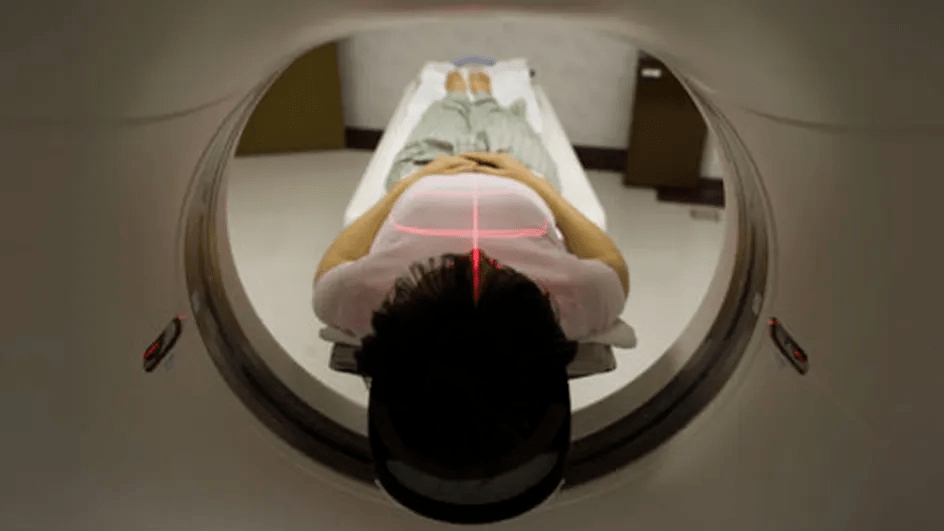
\includegraphics[width=\paperwidth]{Figures/inside_mri.png}}
\begin{frame}[plain]
    % I would like to have the picture of inside the MRI
    % and pass the sound of an MRI scan
    %  \href{run:sons/extract.mp3}{\beamerbutton{écouter}} (https://texnique.fr/osqa/questions/2988/du-son-dans-beamer)
    % https://www.francetvinfo.fr/sante/malgre-l-augmentation-des-besoins-medicaux-le-deficit-en-france-d-appareils-irm-se-fait-de-plus-en-plus-sentir_220301.html
    \href{run:Sounds/mri_sounds.mp3}{\faPlayCircle}
    \begin{minipage}[t][.8\textheight]{\textwidth}    
        \vfill
        
        \tiny
        Credits: \href{https://www.francetvinfo.fr/sante/malgre-l-augmentation-des-besoins-medicaux-le-deficit-en-france-d-appareils-irm-se-fait-de-plus-en-plus-sentir_220301.html}{Getty Images / rubberball}
      \end{minipage}
\end{frame}
}

% link between the 2: this is the sound you hear when undergoing an MRI
% now imagine that you will on average hear this during x minutes
% MRI scanners being slow not only generate discomfort but have other impacts on their efficiency...
\begin{frame}{MRI is slow}
    % for debug
    % This has been run with \TeX~Live~\TeXLiveVersion.
    MRI~(Magnetic Resonance Imaging) scan duration: 15 min (up to 90 min).\footfullcite{nhs}
    \begin{itemize}
        \item discomfort \& accessibility issues
        \item reduced patient throughput
        \item increased motion
    \end{itemize}
    % give typical duration (compare to CT)
    % give associated problems
\end{frame}

\begin{frame}{Our objective: accelerate MRI scans}
    % give TOC
    \setlength{\parskip}{1ex}
    \begin{multicols}{2}
    \tableofcontents
    \end{multicols}
\end{frame}


\section{Introduction to MRI}

\begin{frame}[plain,c]
    %\frametitle{A first slide}
    
    \begin{center}
        \color{DarkBlue}
    \Huge Magnetic Resonance Imaging~(MRI)
    \end{center}
    
\end{frame}

\begin{frame}{What does an MRI look like?}
    \begin{figure}
        \centering
        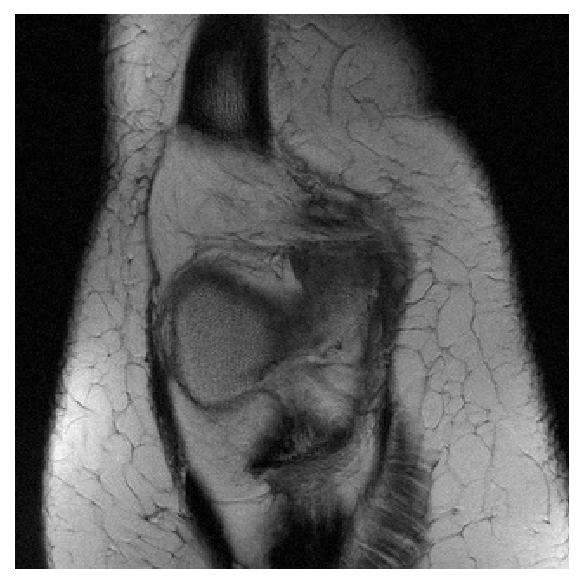
\includegraphics[height=0.6\textheight]{Figures/intro_figures/example_knee_fastmri.pdf}
        \caption{\label{fig:mri-example} \textbf{Example of an MR image}: MR image of the knee taken from the fastMRI dataset.\footfullcite{Zbontar}}
    \end{figure}
\end{frame}

\subsection{Importance of MRI}
\begin{frame}{Importance of MRI - 1}
    % how many MRI scans / scanners
    % how likely is it that you will get an MRI in your life
    % Based on a rough extrapolation of the following figure, there is a 99.9\% chance that you will get an MRI in your life in France.
    99.9\% chance you will get an MRI.
    \begin{figure}
        \centering
        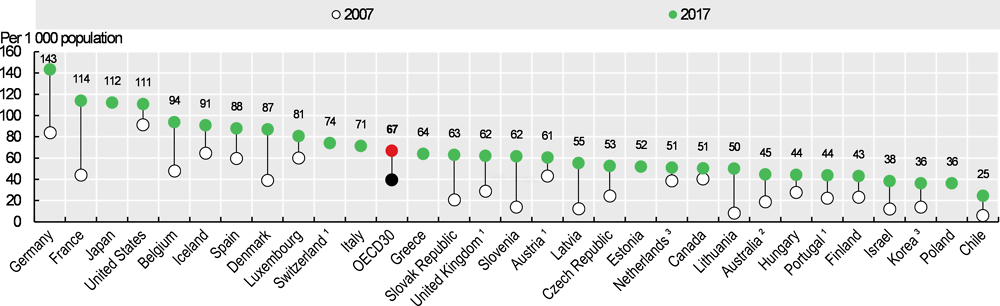
\includegraphics[width=\textwidth]{Figures/intro_figures/num_mri_scans.png}
        \caption{\label{fig:num-mri-scans} \textbf{Number of MRI scans per year per 1000 population}: figure courtesy of \citet{OECDMRI}.}
    \end{figure}
\end{frame}

% There is a reason for that: MRI can help diagnose many different conditions
\begin{frame}{Importance of MRI - 2}
    % list of conditions
    % This illustration provides a non-exhaustive list of all the diagnoses that can be carried out with MRI.
    \begin{figure}
        \centering
        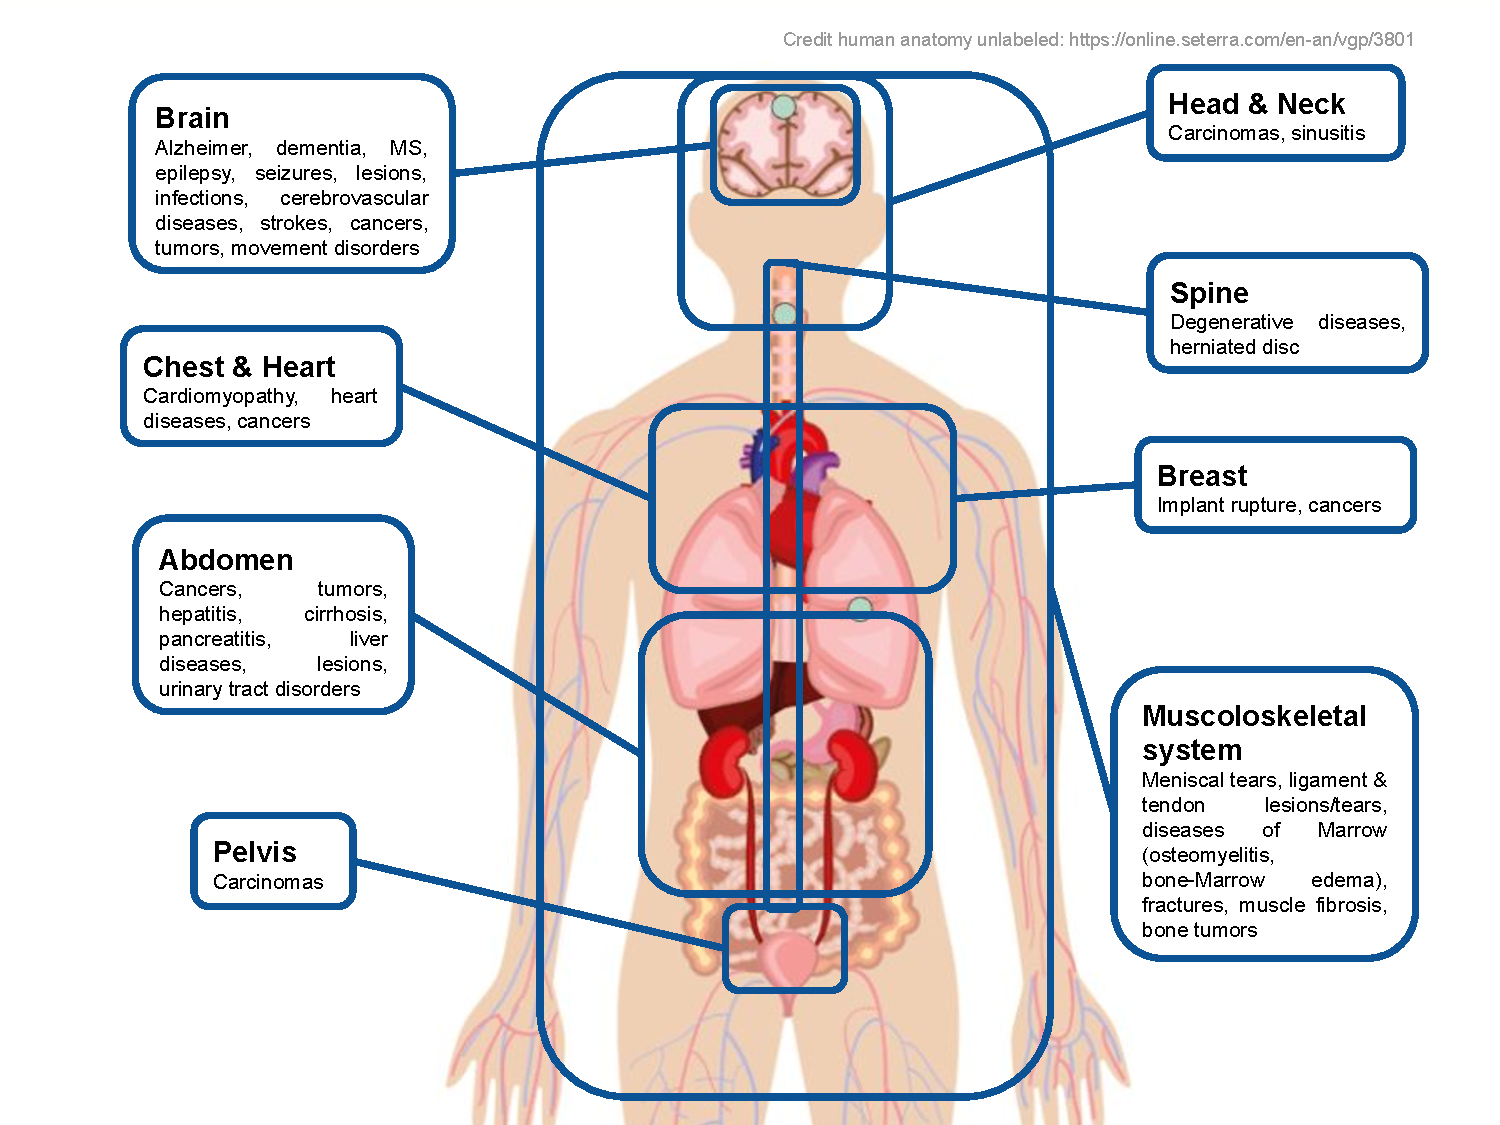
\includegraphics[height=0.6\textheight]{Figures/intro_figures/What_can_we_diagnose_with_MRI.pdf}
        \caption{\label{fig:diagnose-mri} \textbf{What can we diagnose with MRI?}  Info compiled from \citet{reimer2010clinical,runge2019essentials}.}
    \end{figure}
\end{frame}

\subsection{Physics of MRI}
% MRI is so popular why isnt it solved already ?
\begin{frame}{Physics of MRI - 1}
    % at its core MRI relies on the MR phenomenon
    % in short: a spin is aligned with the magnetic field, when an RF pulse is sent, it tips the spin in the orthogonal plane before the spin realigns with the magnetic field sending another RF pulse
    \only<1>{
        \vspace{0.5em}

    \begin{figure}
        \centering
        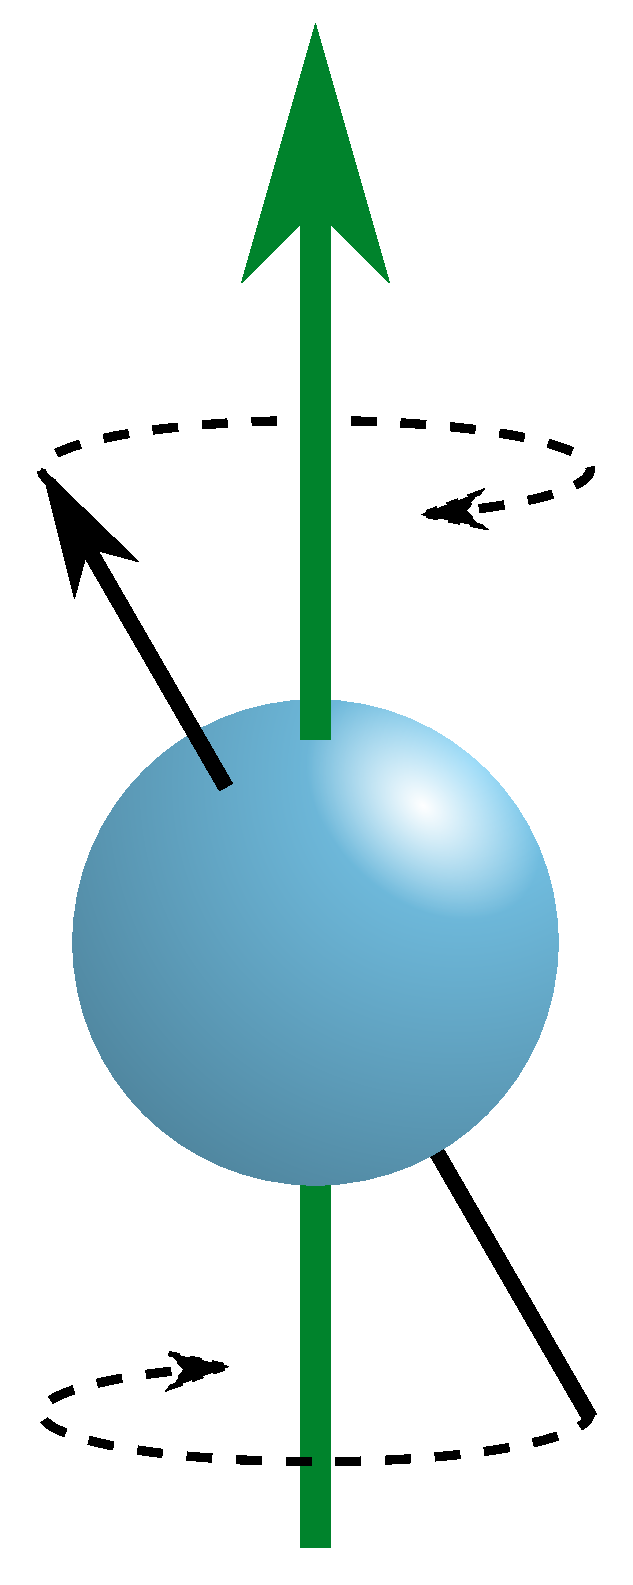
\includegraphics[width=0.14\textwidth]{Figures/intro_figures/Precession_in_magnetic_field.pdf}
        \caption{\label{fig:precession}\textbf{Illustration of the precession of a spin in a magnetic field:} the green arrow represents the $\Bb_0$ magnetic field, while the black arrow represents the magnetic moment of the particle. Illustration courtesy of \citet{wiki}.}
    \end{figure}
    }
    \only<2>{
    \begin{figure}
        \centering
        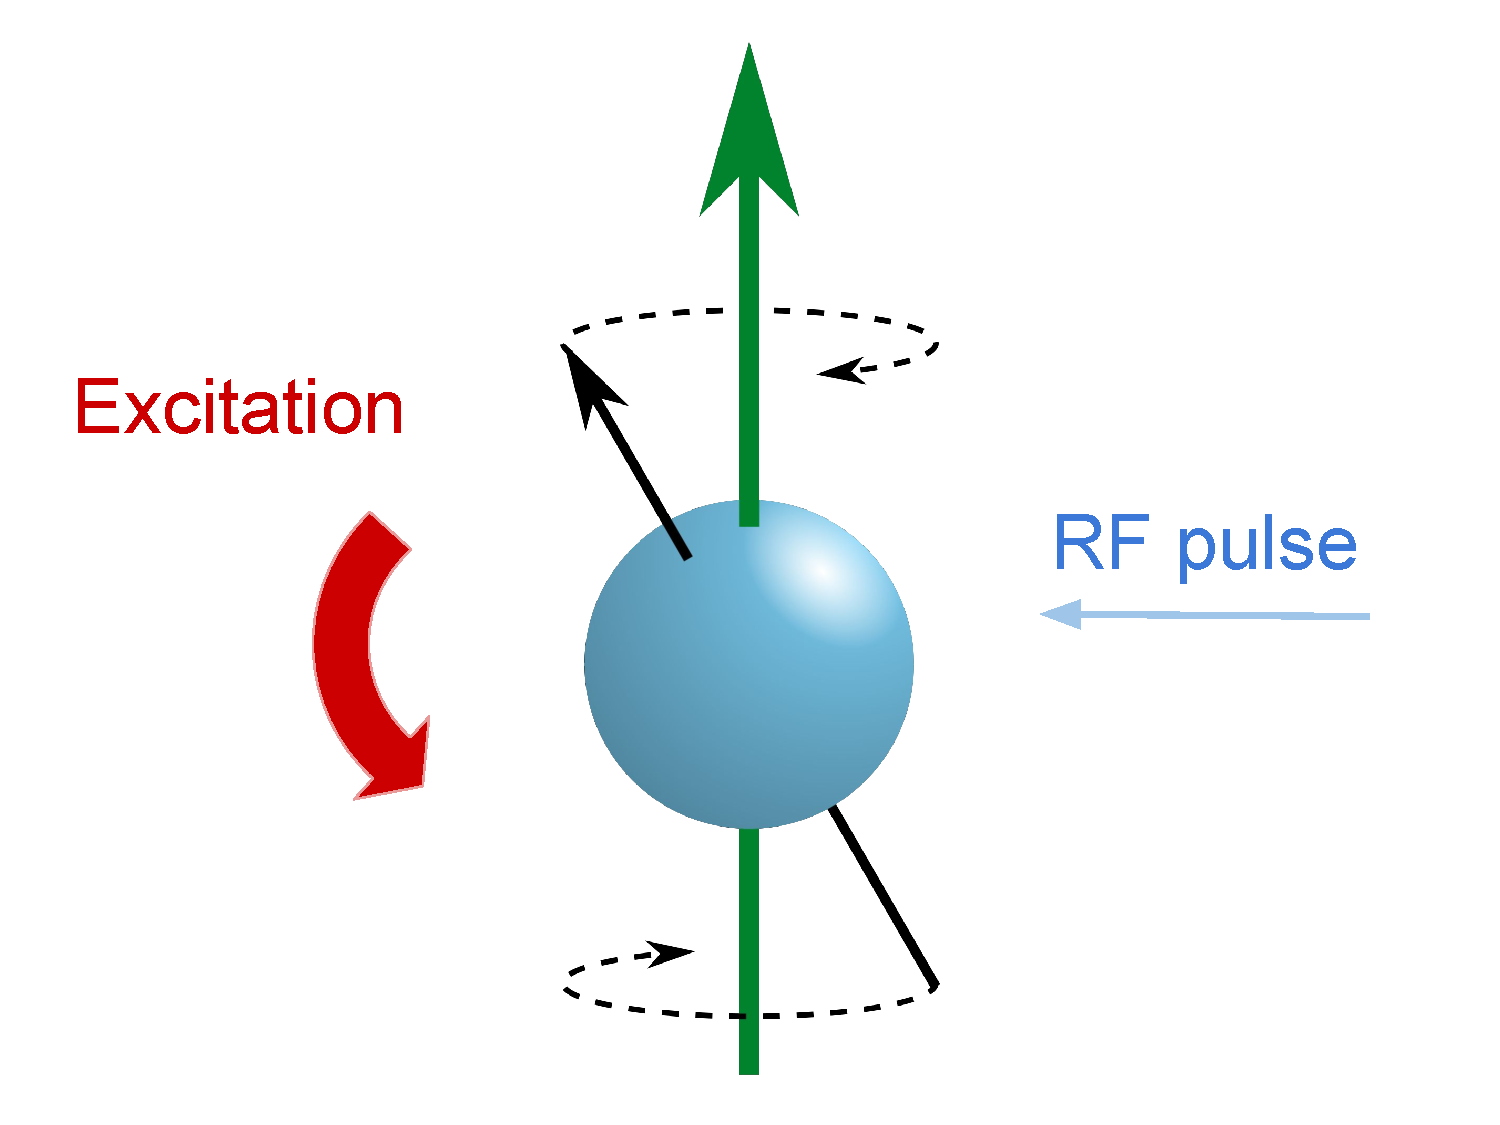
\includegraphics[width=0.5\textwidth]{Figures/intro_figures/Excitation.pdf}
        \caption{\label{fig:excitation}\textbf{Illustration of the excitation phenomenon:} the blue arrow represents an incoming RF~(Radio Frequency) pulse. Illustration courtesy of \citet{wiki}.}
    \end{figure}
    }
    \only<3>{
    \begin{figure}
        % XXX: add antenna for reception of the pulse
        \centering
        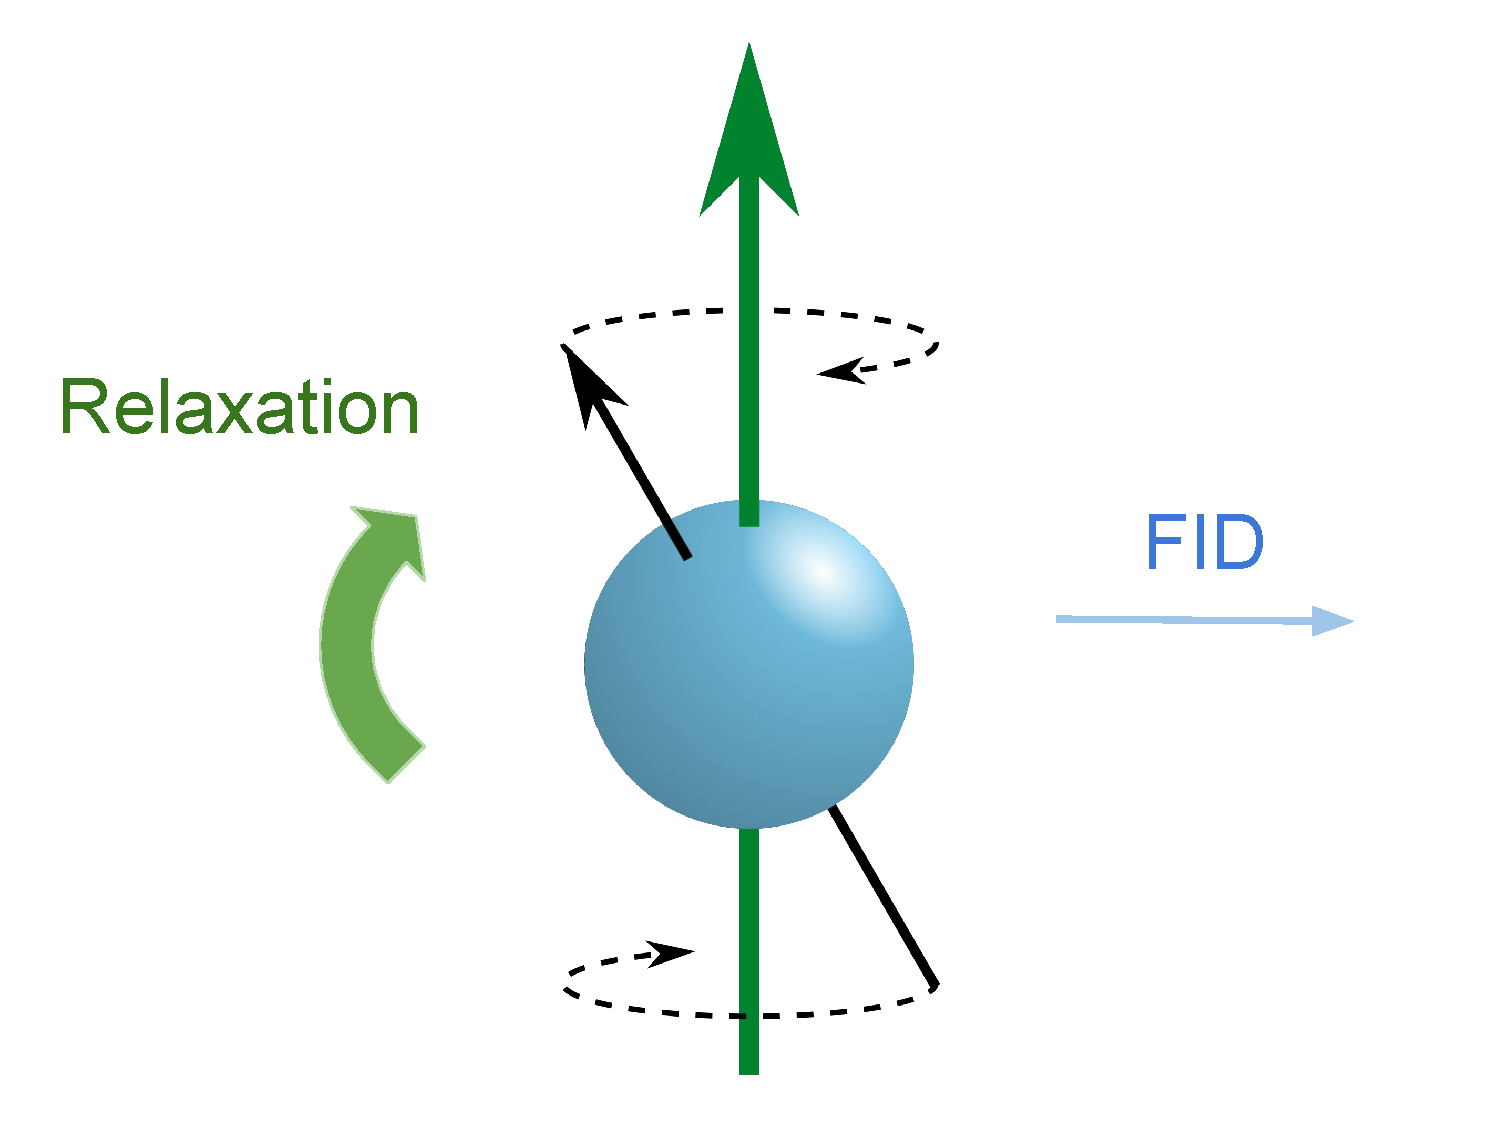
\includegraphics[width=0.5\textwidth]{Figures/intro_figures/Relaxation.pdf}
        \caption{\label{fig:relaxation}\textbf{Illustration of the relaxation phenomenon:} the blue arrow represents an outgoing FID~(Free Induction Decay) pulse. Illustration courtesy of \citet{wiki}.}
    \end{figure}
    }
\end{frame}

\begin{frame}{Physics of MRI - 2}
    % Because all spins get excited, we get a global RF pulse that is the weighted sum of the contribution of all spins' relaxation RF pulses: global information
    % We can obtain "multiple global information", by changing a bit the magnetic field spatially using gradients
    % Signal equation
    % However, the FID carries global information.
    FID: global info.
    \pause
    
    % Using magnetic \textbf{gradients} enables changing a bit the magnetic field spatially, and therefore changing the global information depending on local factors.
    Magnetic \textbf{gradients} $\Rightarrow$ change the magnetic field spatially.
    \pause
    
    % This allows us to receive a temporal signal of the form:
    Temporal signal:
    \begin{equation*}
        \vspace{\baselineskip}
        \tikzmarknode{S}{\highlight{blue}{$S_{tr}(t)$}} \propto \omega_0  \int_{V_s} B_{tr} \tikzmarknode{M}{\highlight{green}{$M_{tr}(t, \rb)$}} e^{-\imath \gamma \rb \cdot \int_0^t \tikzmarknode{G}{\highlight{red}{$\Gb(\tau)$}}  \dif \tau} \dif \rb 
    \end{equation*}
    \begin{tikzpicture}[overlay,remember picture,>=stealth,nodes={align=left,inner ysep=1pt},<-]
        % For "S"
        \onslide<4->{
        \path (S.south) ++ (0,-2em) node[anchor=south east,color=blue!67] (exp_S){\textbf{Recorded MR signal}};
        \draw [color=blue!87](S.south) |- ([xshift=-0.3ex,color=blue]exp_S.south west);
        }
        % For "M"
        \onslide<5->{
        \path (M.south) ++ (0, -6em) node[anchor=south east,color=green!77] (exp_M){\textbf{Magnetic field in each location $\rb$,}\\ \textbf{proportional to the spin density $\rhob(\rb)$}};
        \draw [color=green!87](M.south) |- ([xshift=-0.3ex,color=green]exp_M.south west);
        }
        % For "G"
        \onslide<6->{
        \path (G.south) ++ (0, -2em) node[anchor=north west,color=red!47] (exp_G){\textbf{Temporal gradients,}\\\textbf{controlled by the operator}};
        \draw [color=red!87](G.south) |- ([xshift=-0.3ex,color=red]exp_G.south east);
        }
    \end{tikzpicture}
\end{frame}

\begin{frame}{Physics of MRI - 3}
    % Signal equation $\Rightarrow$ k-space
    % The \textbf{k-space} vector, $\kb(t) = \frac{\gamma}{2\pi} \int_0^t \Gb(\tau) \dif \tau$, defines how we traverse the Fourier space of the anatomical image.
    \textbf{k-space} vector: $\kb(t) = \frac{\gamma}{2\pi} \int_0^t \Gb(\tau) \dif \tau$.

    % We are sampling in the Fourier space of the anatomical image
    %     \caption{\label{fig:example-kspace}\textbf{Example of a k-space with its corresponding anatomical image}: The raw data is from the fastMRI dataset. The k-space is in log-scale and only the magnitude of the 2 images are represented. We selected only a single coil from the 16 coils available for illustrative purposes.}

    \begin{center}
        \begin{tikzpicture}
            \node (kspace) {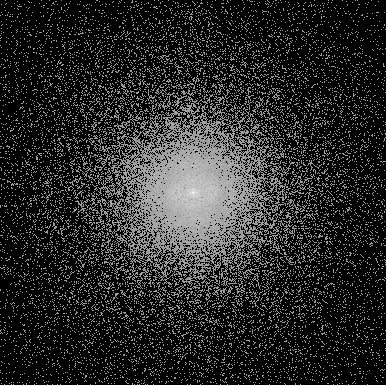
\includegraphics[width=0.31\textwidth]{Figures/intro_figures/kspace_phantom.png}};
            \node[below=0.7em of kspace] (kspace_exp) {$\kb(t)$};
            \node[right=of kspace] (brain) {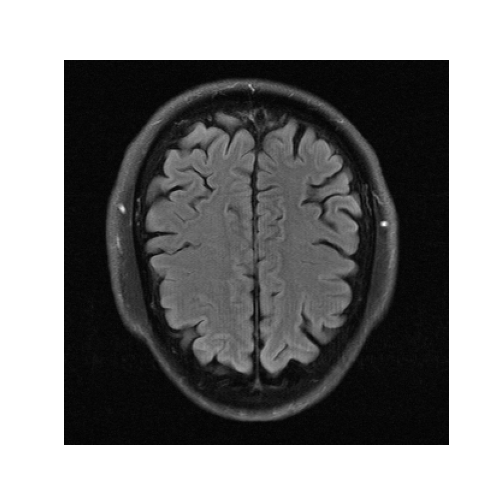
\includegraphics[width=0.4\textwidth, angle=180]{Figures/intro_figures/image_gt (2).png}};
            \draw[-{Triangle[width=18pt,length=8pt]}, line width=10pt, draw=blue!57](kspace.east) -- node [midway,above] {IFFT} ($(brain.west)+(1.6em, 0)$);
        \end{tikzpicture}
    \end{center}
\end{frame}

\begin{frame}{Physics of MRI - 4}
    % Let's not forget our initial goal here: we want to understand why MRI is slow
    % The relaxation is slow !
    \begin{block}{Recap}
        MRI relies on the nuclear resonance phenomenon. This enables us to sample the Fourier space of the anatomical object of interest.
    \end{block}
    \pause
    MRI is slow, because the \textbf{relaxation} is slow!
\end{frame}

\subsection{Acceleration in MRI}
\begin{frame}{Where is there room for acceleration?}
    % Explain the concept of redundancy
    % first example: partial Fourier $\Rightarrow$ give limits
    % \textbf{Redundancy}, otherwise called \textbf{sparsity, symmetry, structure or a priori information}, is the core concept that will help us accelerate MRI.\\
    \textbf{Redundancy}, or \textbf{sparsity, symmetry, structure or a priori information}, is the key.\\
    
    \begin{overprint}
        \onslide<2>
        \hfill \break
    % Here is an illustrative example:
    An illustrative example:
    \begin{figure}
        \centering
        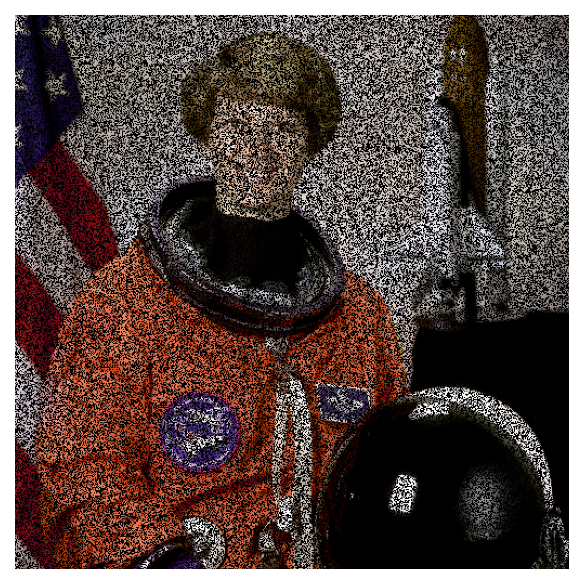
\includegraphics[height=0.4\textheight]{Figures/intro_figures/astronaut_masked.pdf}
        \caption{\label{fig:astronaut-masked}\textbf{The inpainting problem.} 
        % Even without access to all the pixel values directly, we can infer them, because the information in the image is redundant.
        }
    \end{figure}
    
    \onslide<3>
    \hfill \break
    An illustrative example:
    \begin{figure}
        \centering
        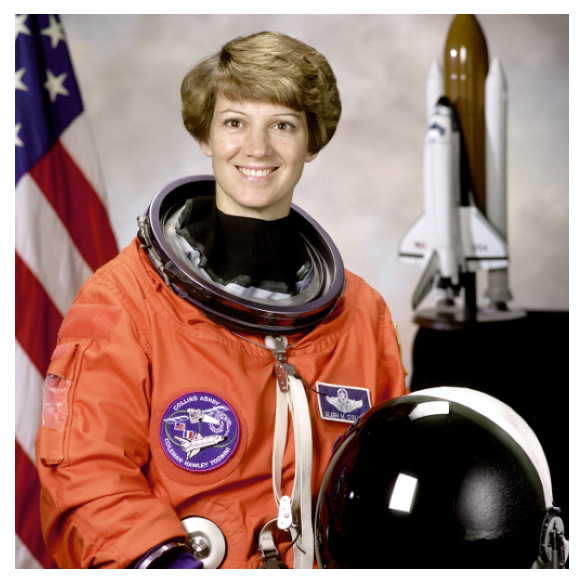
\includegraphics[height=0.4\textheight]{Figures/intro_figures/astronaut.pdf}
        \caption{\label{fig:astronaut}\textbf{The inpainting problem.} 
        % Even without access to all the pixel values directly, we can infer them, because the information in the image is redundant.
        }
    \end{figure}
    
    \onslide<4>
        \hfill \break
        Is there a similar thing in MRI?

        % Yes! The anatomical image is real-valued so its Fourier Transform~(FT) has a conjugate symmetry.
        Yes! Fourier Transform~(FT) has a conjugate symmetry $\Rightarrow$ \textbf{Partial Fourier}
        % Using this redundancy to sample less points in the k-space (i.e. using the relaxation fewer times) is a technique called \textbf{Partial Fourier}.
        
        % But in practice it is still needed to sample 6/8 of the Fourier space (acceleration of 1.3).\footfullcite{emri}
        Resulting acceleration: 1.3
    
    \end{overprint}
    
\end{frame}

\begin{frame}{Parallel imaging}
    % "forging" the redundancy
    % We can build more redundancy in the measuring system by using \textbf{more antennas (called coils)} to measure the magnetic signal.
    More redundancy using \textbf{more antennas (called coils)} $\Rightarrow$ \textbf{Parallel Imaging~(PI)}
     
    % This technique is called \textbf{Parallel Imaging~(PI)}. 
    % A reconstruction algorithm is now needed to handle the multi-coil undersampled data.
        % \textbf{SENSE}\footfullcite{Pruessmann1999SENSE:MRI} and \textbf{GRAPPA}\footfullcite{Griswold2002GeneralizedGRAPPA} are such algorithms.    
    Multi-coil reconstruction algorithm: \textbf{SENSE}\footfullcite{Pruessmann1999SENSE:MRI} and \textbf{GRAPPA}\footfullcite{Griswold2002GeneralizedGRAPPA}.
    % GRAPPA + SENSE examples
\end{frame}

\begin{frame}{The example of GRAPPA}
    \begin{figure}
        \centering
        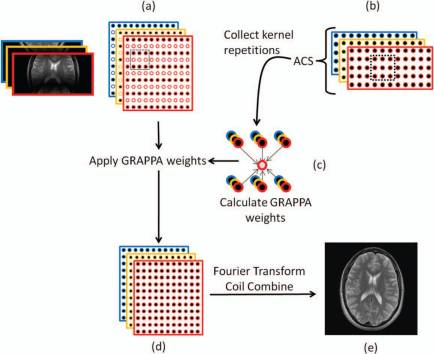
\includegraphics[height=0.6\textheight]{Figures/intro_figures/GRAPPA.jpeg}
        \caption{\label{fig:GRAPPA}\textbf{GRAPPA illustration.} Image courtesy of \citet{deshmane2012parallel}.
        }
    \end{figure} 
\end{frame}

\begin{frame}{Limits of Parallel Imaging}
    % Max AF
    Resulting acceleration: 2
    % ow: https://www.siemens-healthineers.com/magnetic-resonance-imaging/options-and-upgrades/clinical-applications/syngo-grappa says 2,3
\end{frame}
% cSpell: disable
\section{Inverse Problems}

\begin{frame}[plain,c]
    %\frametitle{A first slide}

    \begin{center}
        \color{DarkBlue}
    \Huge \thesection. \insertsection
    \end{center}

\end{frame}

\begin{frame}{Linear Inverse Problems}
    % introduce linear inverse problems
    % To leverage this type of redundancy, we introduce the concept of \textbf{Linear Inverse Problems}:
    % \textbf{Linear Inverse Problems}:
    \begin{equation*}
        \tikzmarknode{A}{\highlight{green}{$\Ab$}} \tikzmarknode{x}{\highlight{blue}{$\xb$}} = \tikzmarknode{y}{\highlight{yellow}{$\yb$}}
    \end{equation*}
    \vspace{2.5\baselineskip}
    \begin{tikzpicture}[overlay,remember picture,>=stealth,nodes={align=left,inner ysep=1pt},<-]
        % For "A"
        \onslide<6>{
        \path (A.south) ++ (0,-2em) node[anchor=south east,color=DarkGreen!77] (exp_A){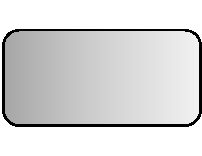
\includegraphics[width=0.05\textwidth]{Figures/intro_figures/smiley_prior_forw_op.pdf}};
        \draw [color=DarkGreen!87](A.south) |- ([xshift=-0.3ex,color=DarkGreen]exp_A.south west);
        }
        \onslide<7->{
        \path (A.south) ++ (0,-2em) node[anchor=south east,color=DarkGreen!77] (exp_A){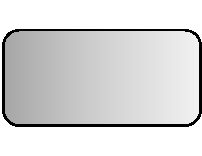
\includegraphics[width=0.05\textwidth]{Figures/intro_figures/smiley_prior_forw_op.pdf} \textbf{Measurement operator}};
        \draw [color=DarkGreen!87](A.south) |- ([xshift=-0.3ex,color=DarkGreen]exp_A.south west);
        }
        % For "x"
        \onslide<2>{
            \path (x.south) ++ (0, -4.5em) node[anchor=south east,color=blue!67] (exp_x){
\includegraphics[width=0.05\textwidth]{Figures/intro_figures/smiley_prior_x.pdf}};
        \draw [color=blue!87](x.south) |- ([xshift=-0.3ex,color=blue]exp_x.south west);
        }
        \onslide<3->{
        \path (x.south) ++ (0, -4.5em) node[anchor=south east,color=blue!67] (exp_x){
\includegraphics[width=0.05\textwidth]{Figures/intro_figures/smiley_prior_x.pdf} \textbf{Signal to reconstruct}};
        \draw [color=blue!87](x.south) |- ([xshift=-0.3ex,color=blue]exp_x.south west);
        }
        % For "y"
        \onslide<4>{
            \path (y.south) ++ (0, -1em) node[anchor=north west,color=amber!67] (exp_y){
\includegraphics[width=0.05\textwidth]{Figures/intro_figures/smiley_prior_y.pdf}};
            \draw [color=amber!87](y.south) |- ([xshift=-0.3ex,color=amber]exp_y.south east);
        }
        \onslide<5->{
        \path (y.south) ++ (0, -1em) node[anchor=north west,color=amber!67] (exp_y){
\includegraphics[width=0.05\textwidth]{Figures/intro_figures/smiley_prior_y.pdf} \textbf{Measurements}};
        \draw [color=amber!87](y.south) |- ([xshift=-0.3ex,color=amber]exp_y.south east);
        }
    \end{tikzpicture}


    \onslide<8->{
    % Problems arise when $\ker{\Ab} \neq \{0\}$, i.e. when there are multiple solutions to this equation.
    Problem: Multiple solutions! Formally $\ker{\Ab} \neq \{0\}$.
    }

    \onslide<9->{
    \hfill \break
    % In order to select one of these solutions, we need to use a priori knowledge.
    To select one of these solutions, we need a priori knowledge.
    }
\end{frame}

\begin{frame}{Another look at redundancy: the prior point of view}
    % give a sense of what structure is and how it relates to redundancy
    % Redundancy is not always strict: we may only have a strong correlation between 2 structures of the image.
    Redundancy is not always strict
    \only<1>{
        \begin{figure}
            \centering
            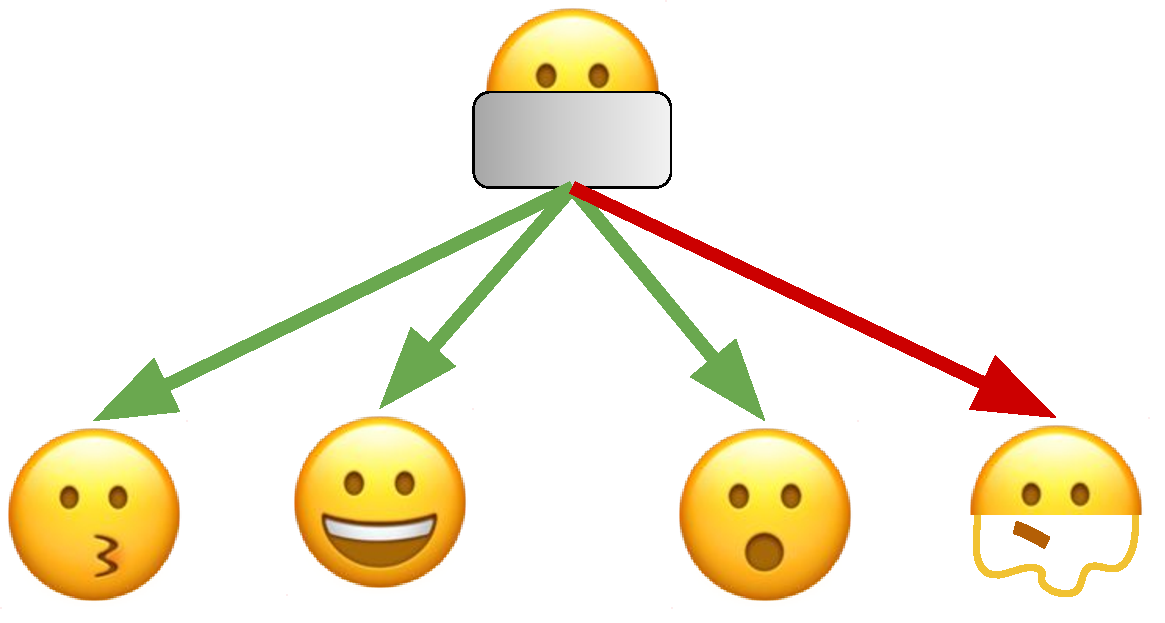
\includegraphics[height=0.5\textheight]{Figures/cs_figures/smiley_prior.pdf}
            \caption{\label{fig:redundancy-smiley}\textbf{A smiley example to a priori knowledge.}
            % Even if we do not have access to the whole image, we still know which images are more \emph{likely} to correspond to it.
            }
        \end{figure}
    }
    \only<2->{
        \begin{center}
            \begin{tikzpicture}[font=\large,>=stealth,node distance=1.5em, remember picture]
                % node
                \node(f_smiley) {$\tikzmarknode{f}{f}\left(\adjincludegraphics[valign=c,width=0.1\textwidth]{Figures/intro_figures/smiley_prior_x.pdf}\right) = $};
                \node(arrow) [right=of f_smiley.east, single arrow,bottom color=red,top color=green, minimum size=2cm,rotate=90, yshift=-1em, xshift=-1em] {};
                \node(likely_smiley) [above=0.2em of arrow.east] {Smiley-like};
                \node(unlikely_smiley) [below=0.2em of arrow.west] {Not smiley-like};
                \node(f_exp) [below=of f, visible on=<3>] {Prior};
                % arrow
                \draw<3-> [line width=0.1em] ($(f.south)+(0,-0.1cm)$) -- (f_exp.north);
            \end{tikzpicture}
        \end{center}
    }
\end{frame}



\begin{frame}{Application to MRI}
    % MR images themselves cannot be represented as sparse vectors directly, we need a way to express them as such.
    % MR images are not sparse as is.
    % \citet{Lustig2007} did that by using the fact that MR images can be represented sparsely in a \textbf{wavelet} basis.
    % \citet{Lustig2007} expressed their sparsity in a \textbf{wavelet} basis.

    \hfill \break
    The Inverse Problem becomes:
    \begin{equation*}
        \tikzmarknode{FS}{\highlight{green}{$\left(\Ib_L\otimes {\mathcal{F}}_{\Omega}\right)\Sbb$}} \tikzmarknode{x}{\highlight{blue}{$\xb$}} = \tikzmarknode{y}{\highlight{yellow}{$\ybb$}}
    \end{equation*}
    \begin{tikzpicture}[overlay,remember picture,>=stealth,nodes={align=left,inner ysep=1pt},<-]
        % For "FS"
        \onslide<4>{
        \path (FS.south) ++ (0,-4em) node[anchor=south east,color=DarkGreen!77,align=right] (exp_FS){
            \textbf{$\mathcal{F}_{\Omega}$ : FT on the $\Omega$ set;}\\
            \textbf{$\Sbb=[\Sb_1^H,\ldots, \Sb_L^H]^\top$: the sensitivity maps}\\
            \textbf{per coil}
        };
        \draw [color=DarkGreen!87](FS.south) |- ([xshift=-0.3ex,color=DarkGreen]exp_FS.south west);
        }
        \onslide<5>{
        \path (FS.south) ++ (0,-4em) node[anchor=south east,color=DarkGreen!77] (exp_FS){
            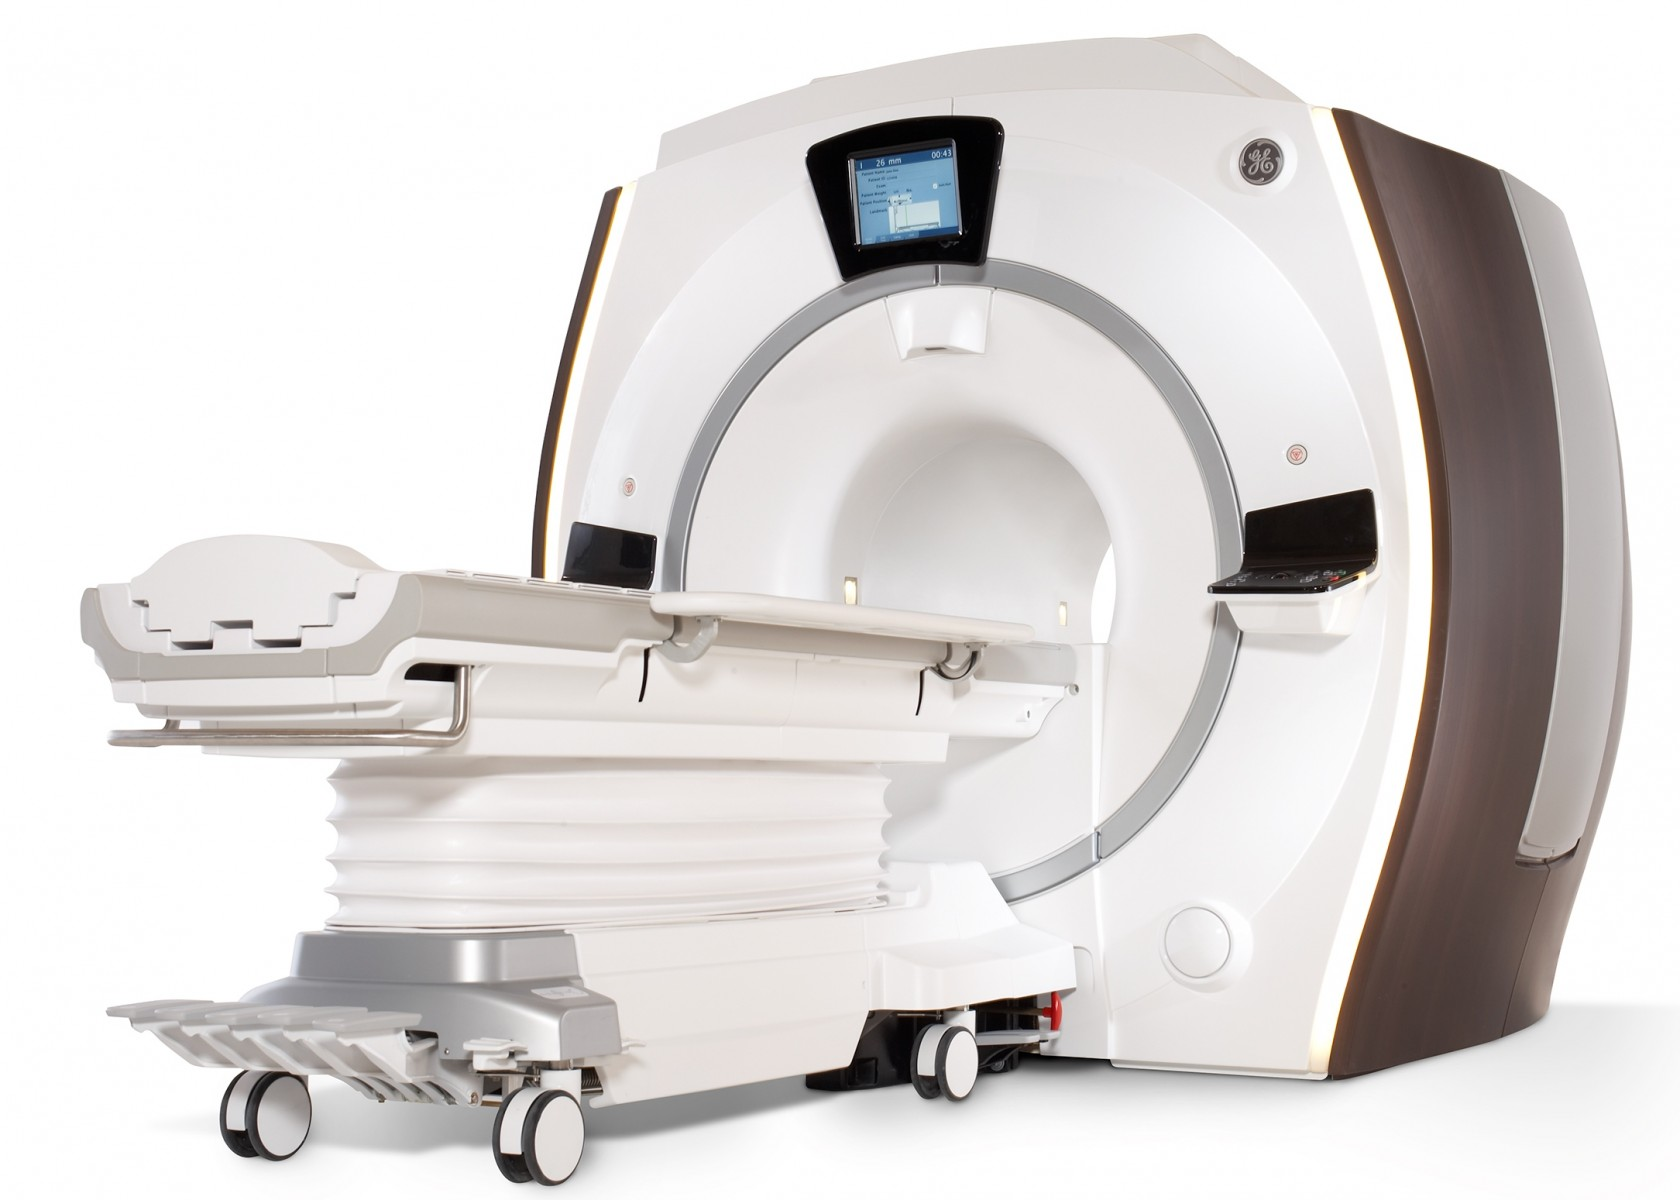
\includegraphics[width=0.1\textwidth]{Figures/intro_figures/mri.jpg}
        };
        \draw [color=DarkGreen!87](FS.south) |- ([xshift=-0.3ex,color=DarkGreen]exp_FS.south west);
        }
        % For "x"
        \onslide<2-4>{
        \path (x.south) ++ (0, -2em) node[anchor=south west,color=blue!67] (exp_x){\textbf{2D or 3D MR image $\in \mathbb{C}$}};
        \draw [color=blue!87](x.south) |- ([xshift=-0.3ex,color=blue]exp_x.south east);
        }
        \onslide<5->{
        \path (x.south) ++ (0, -4em) node[anchor=south west,color=blue!67] (exp_x){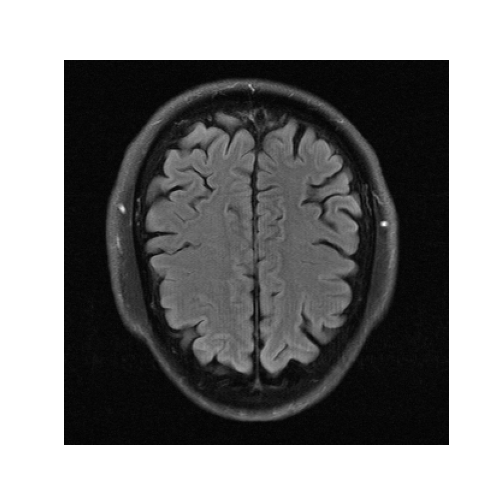
\includegraphics[width=0.1\textwidth]{Figures/intro_figures/brain_mri.png}};
        \draw [color=blue!87](x.south) |- ([xshift=-0.3ex,color=blue]exp_x.south east);
        }
        % For "y"
        \onslide<3-4>{
        \path (y.north) ++ (0, 1em) node[anchor=south west,color=amber!67] (exp_y){$\ybb=[\yb_1^H, \ldots, \yb_L^H]^\top$,\\ \textbf{k-space measurements} \\ \textbf{for each coil}};
        \draw [color=amber!87](y.north) |- ([xshift=-0.3ex,color=amber]exp_y.south east);
        }
        \onslide<5->{
        \path (y.north) ++ (0, 1em) node[anchor=south west,color=amber!67] (exp_y){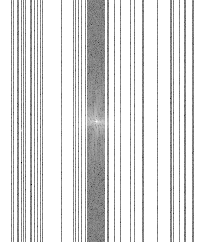
\includegraphics[width=0.07\textwidth]{Figures/intro_figures/kspace_mri.png}};
        \draw [color=amber!87](y.north) |- ([xshift=-0.3ex,color=amber]exp_y.south east);
        }
    \end{tikzpicture}

    \onslide<4>{
        \vspace{4em}
        $\Omega$: Cartesian when on a uniform grid, non-Cartesian otherwise.

        $\Sbb$: 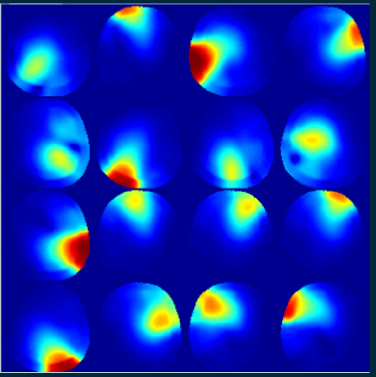
\includegraphics[height=0.2\textheight]{Figures/cs_figures/smaps.png}
    }
\end{frame}

% \begin{frame}{Relaxation}
%     Can we solve the optimization problem?
%     \pause
%     No; we need to relax it using the basis pursuit:
%     \begin{equation*}
%         \label{eq:basis-pursuit}
%         \min_{\xb \in \mathbb{C}^n} \|\xb\|_1 \quad \text{subject to} \quad \Ab \xb = \yb
%     \end{equation*}

%     \pause
%     % For this problem to have the same solutions as the non-relaxed one, we need coherence-based constraints on the measurement operator $\Ab$.
%     Coherence-based constraints on $\Ab$ $\Rightarrow$ same solutions.

% \end{frame}

\begin{frame}{The canonical MRI reconstruction problem}
    % We introduce the notion of a \textbf{sparsity} basis $\psib$ (typically wavelets) and the fact that the measurements can be noisy to obtain the canonical MRI reconstruction problem:
    \begin{equation*}
        \argmin_{\xb \in \mathbb{C}^n} \overbrace{\frac12 \|\tikzmarknode{calA}{\highlight{green}{$\mathcal{A}$}} \xb - \yb \|_2^2}^{\text{\sf \footnotesize Noisy data consistency}}  + \overbrace{ \tikzmarknode{lambda}{\underline{\lambda}} \|\tikzmarknode{psi}{\highlight{brown}{$\psib$}} \xb\|_1}^{\text{\sf \footnotesize Regularization term, $\mathcal{R}$ } }
    \end{equation*}
    \vspace{\baselineskip}
    \begin{tikzpicture}[overlay,remember picture,>=stealth,nodes={align=left,inner ysep=1pt},<-]
        % For "calA"
        \path (calA.south) ++ (0,-2.5em) node[anchor=south east,color=DarkGreen!87] (exp_calA){
            $= \left(\Ib_L\otimes {\mathcal{F}}_{\Omega}\right)\Sbb$
        };
        \draw [color=DarkGreen!87](calA.south) |- ([xshift=-0.3ex,color=DarkGreen]exp_calA.south west);
        % For psi
        \path (psi.south) ++ (0, -2.5em) node[anchor=south west,color=brown!87] (exp_psi){
            Wavelet basis
        };
        \draw [color=brown!87](psi.south) |- ([xshift=-0.3ex,color=brown]exp_psi.south east);
        % For "lambda"
        \path (lambda.south) ++ (0, -4.5em) node[anchor=south west,color=black!87] (exp_lambda){
            Regularization hyperparameter
        };
        \draw [color=black!87](lambda.south) |- ([xshift=-0.3ex,color=black]exp_lambda.south east);
    \end{tikzpicture}
    \footnotetext{\fullcite{Lustig2007}}
\end{frame}

% \begin{frame}{ISTA}
%     %  The Iterative Shrinkage-Thresholding Algorithm~(ISTA) can be used to solve the canonical MRI reconstruction problem:
%      Iterative Shrinkage-Thresholding Algorithm~(ISTA):
%      % XXX: already highlight the steps to have a visual understanding
%      \begin{equation*}
%         \label{eq:ista-step}
%         \begin{split}
%             \xb_{n+1} &= \highlight{yellow}{$\xb_n - \epsilon_n \mathcal{A}^H\left(\mathcal{A} \xb_n - \ybb\right)$}\\
%             \xb_{n+1} &= \highlight{blue}{$\tikzmarknode{prox}{\operatorname{prox}}_{\epsilon_n \tikzmarknode{reg}{\mathcal{R}}}\left(\xb_{n+1}\right)$}
%         \end{split}
%     \end{equation*}
%     \begin{tikzpicture}[overlay,remember picture,>=stealth,nodes={align=left,inner ysep=1pt},<-]
%         % For "prox"
%         \path (prox.south) ++ (0,-2.5em) node[anchor=south east,color=black!87] (exp_prox){
%             Proximity operator
%         };
%         \draw [color=black!87](prox.south) |- ([xshift=-0.3ex,color=black]exp_prox.south west);
%         % For "reg
%         \path (reg.south) ++ (0, -2.5em) node[anchor=south west,color=black!87] (exp_reg){
%             \footnotesize $= \|\psib \cdot\|_1$
%         };
%         \draw [color=black!87](reg.south) |- ([xshift=-0.3ex,color=black]exp_reg.south east);
%     \end{tikzpicture}
% \end{frame}

% \begin{frame}{Dictionary Learning}

% \end{frame}


\begin{frame}{Limitations of classical recovery algorithms}
    % give max AF
    % also give a sense of the limitations in compute and in prior learning
    Additional acceleration factor on top of PI: 1.5. % from https://www.philips.fr/healthcare/ressources/landing/the-next-mr-wave/compressed-sense

    \pause
    The prior knowledge expressed by the wavelet basis (or other basis) is limited: handcrafted and linear.
\end{frame}

\begin{frame}{Compressed Sensing}
    \begin{block}{Recap}
        MRI is slow because of \textbf{relaxation}.

        \pause
        We can use \textbf{redundancy} in many forms to reduce the amount of samples we need in the Fourier space, and therefore the number of relaxations.

        \pause
        But we are limited by simple forms of redundancy.
    \end{block}
\end{frame}


\addtocontents{toc}{\newpage}

\section{Deep Learning}

\begin{frame}[plain,c]
    %\frametitle{A first slide}
    
    \begin{center}
        \color{DarkBlue}
    \Huge \insertsection
    \end{center}
    
\end{frame}

\begin{frame}{The power of Deep Learning}
    % we want to learn a complicated function that tells us whether an image is an MR image
    % similarly deep learning has been able to build functions that tell whether an image is that of a dog or a cat
    % universal approx
    % We want to learn a complicated function that tells us whether a complex-valued vector is an MR image or not.
    % We want a function that tells us whether a vector is an MR image or not.
    The prior is a complicated visual function.
    \pause

    Deep Learning~(DL) has been used to build complicated functions:
    {\Large
        \begin{equation*}
            \tikzmarknode{nn}{\highlight{brown}{$f_\thetab$}}\left( \adjincludegraphics[valign=c,width=0.2\textwidth]{Figures/intro_figures/chowchow.jpg} \right) = \text{"DOG"}
        \end{equation*}
        \begin{tikzpicture}[overlay,remember picture,>=stealth,nodes={align=left,inner ysep=1pt},<-,font=\normalsize]
            % For "nn"
            \onslide<3->{
            \path (nn.south) ++ (0, -4.5em) node[anchor=south west,color=brown!87] (exp_nn){
                Neural network:\\a chain of elementary linear \& nonlinear functions};
            \draw [color=brown!87](nn.south) |- ([xshift=-0.3ex,color=brown]exp_nn.south east);
            }            
        \end{tikzpicture}
    }
\end{frame}

\begin{frame}{Formalism - 1}
    % supervised learning objective function
    % The classical framework for DL is supervised learning:
    Supervised learning:
    \vspace{\baselineskip}

    \begin{equation*}
        \argmin_{\tikzmarknode{params}{\highlight{orange}{$\thetab \in \Theta$}}} \tikzmarknode{sum}{\highlight{purple}{$\sum\limits_{(\xb_i, \yb_i) \in \mathcal{D}}$}} \tikzmarknode{loss}{\highlight{green}{$\mathcal{L}$}}(\tikzmarknode{nn}{\highlight{brown}{$f_{\thetab}$}} (\tikzmarknode{input}{\highlight{blue}{$\xb_i$}}), \tikzmarknode{label}{\highlight{red}{$\yb_i$}}, \thetab)
    \end{equation*}
    % XXX add visual aid to formalism
    \begin{tikzpicture}[overlay,remember picture,>=stealth,nodes={align=left,inner ysep=1pt},<-]
        % For "input"
        \onslide<2->{
        \path (input.north) ++ (0,1.5em) node[anchor=south west,color=blue!87] (exp_input){
            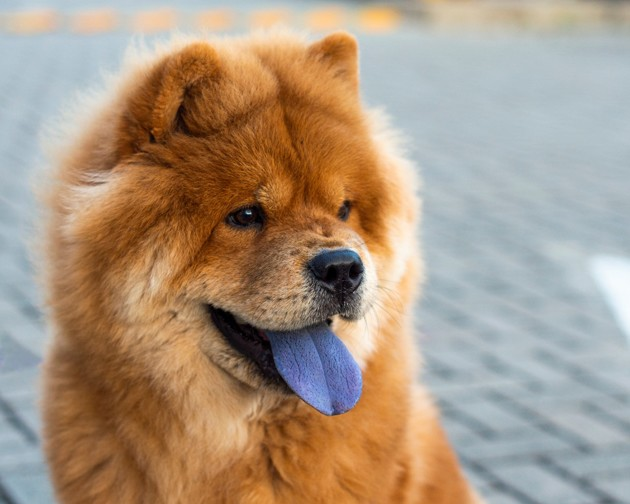
\includegraphics[width=0.05\textwidth]{Figures/intro_figures/chowchow.jpg} input};
        \draw [color=blue!87](input.north) |- ([xshift=-0.3ex,color=blue]exp_input.south east);
        }
        % For "label"
        \onslide<3->{
        \path (label.south) ++ (0, -2.5em) node[anchor=south west,color=red!87] (exp_label){
            "DOG", label};
        \draw [color=red!87](label.south) |- ([xshift=-0.3ex,color=red]exp_label.south east);
        }
        % For "nn"
        \onslide<4->{
        \path (nn.south) ++ (0, -4.5em) node[anchor=south east,color=brown!87] (exp_nn){
            neural network};
        \draw [color=brown!87](nn.south) |- ([xshift=-0.3ex,color=brown]exp_nn.south west);
        }
        % For "loss"
        \onslide<5->{
        \path (loss.north) ++ (0, 1.5em) node[anchor=south west,color=DarkGreen!77] (exp_loss){
            loss};
        \draw [color=DarkGreen!87](loss.north) |- ([xshift=-0.3ex,color=DarkGreen]exp_loss.south east);
        }
        % For "sum"
        \onslide<6->{
        \path (sum.south) ++ (0, -2em) node[anchor=south east,color=purple!87] (exp_sum){
            Estimator of the expected value};
        \draw [color=purple!87](sum.south) |- ([xshift=-0.3ex,color=purple]exp_sum.south west);
        }
        
        % For "params"
        \onslide<7->{
        \path (params.west) ++ (-2em, 0) node[anchor=east,color=orange!87] (exp_params){
            Parameters};
        \draw [color=orange!87](params.west) -- ([xshift=-0.3ex,color=orange]exp_params.east) -- ([xshift=-0.3ex,color=orange]exp_params.south east) -- ([xshift=-0.3ex,color=orange]exp_params.south west);
        }
        
    \end{tikzpicture}
\end{frame}

\begin{frame}{Formalism - 2}
    % Stochastic Gradient descent and chain rule
    To solve the previous equation we will use two main tools:
    
    \begin{enumerate}
        \item \alt<2>{Stochastic Gradient Descent~(SGD)}{\highlight{blue}{Stochastic Gradient Descent~(SGD)}};
        \item<2> \highlight{blue}{Chain rule}.
    \end{enumerate}

    
        \begin{block}{Definition}
            \only<1>{An algorithm to solve the previous optimization problem based on first order derivatives.}
            \only<2>{
                A property allowing us to compute easily derivatives of compound functions.
                \begin{equation*}
                    \frac{\partial f}{\partial y} = \frac{\partial f}{\partial x} \frac{\partial x}{\partial y}
                \end{equation*}
            }
        \end{block}   
    
\end{frame}

\begin{frame}{Requirements for Deep Learning}
    % Great that I can do that, but does it take ?
    % Data, compute + memory, framework
    % accept that it's "black-box"
    What does it take to use DL in a problem?
    \begin{itemize}[<+->]
        \item data
        \item compute \& memory
        \item development framework
        \item accepting that it's "black-box"
    \end{itemize}
\end{frame}

% \begin{frame}{Building the network}
%     % give classical functions
% \end{frame}

\begin{frame}{Introduction Recap}
    \begin{block}{Recap}
        MRI is slow because of \textbf{relaxation}.
        
        \pause
        If we want to do fewer relaxations, we need to exploit some \textbf{redundancy} in MR images.
        
        \pause
        But this redundancy is not easy to express with handcrafted linear functions.
        
        \pause
        This is why we want to use \textbf{Deep Learning} which enables the calibration of complicated functions.
    \end{block}
\end{frame}

% cSpell: disable
\def\qualifigsepigogd{.1mm}
\section{Deep Learning for MRI reconstruction}

\begin{frame}[plain,c]
    %\frametitle{A first slide}

    \begin{center}
        \color{DarkBlue}
    \Huge \thesection. \insertsection
    \end{center}

\end{frame}

% XXX have visual aid in all equations
\begin{frame}{Model agnostic learning}
    % reframing the problem as supervised learning
    % no knowledge of the physics imposed in the model
    % The first use of DL for MRI reconstruction is to actually throw away most of what we just saw:\footfullcite{Zhu2018}
    Let's throw away all we know:\footfullcite{Zhu2018}
    \begin{equation*}
        f_{\thetab}(\measurements) = \imageb
    \end{equation*}
    \begin{tikzpicture}[overlay,remember picture,>=stealth,nodes={align=left,inner ysep=1pt},<-]
        % For "kspace"
        \onslide<2->{
        \path (kspace.south) ++ (0,-5em) node[anchor=south east,color=amber!87] (exp_kspace){
            \textbf{kspace} 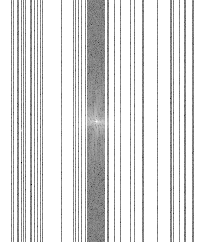
\includegraphics[width=0.1\textwidth]{Figures/intro_figures/kspace_mri.png}};
        \draw [color=amber!87](kspace.south) |- ([xshift=-0.3ex,color=amber]exp_kspace.south west);
        }
        % For "image"
        \onslide<3->{
        \path (image.south) ++ (0, -4.3em) node[anchor=south west,color=blue!87] (exp_image){
            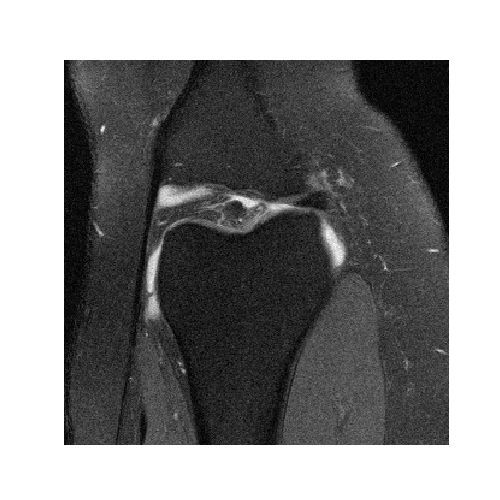
\includegraphics[width=0.1\textwidth,trim=3.3em 3.3em 3.3em 3.3em,clip]{Figures/dl_mri_figures/gt_knee.png} \textbf{image}};
        \draw [color=blue!87](image.south) |- ([xshift=-0.3ex,color=blue]exp_image.south east);
    }
    \end{tikzpicture}

    \onslide<4->{
        \vspace{3em}
        Cons:
    \begin{itemize}
        \item Not taking advantage of our knowledge of the physics
        \item No scaling
    \end{itemize}
    }
\end{frame}

\begin{frame}{Single domain learning}
    % Use the backward operator as a basis for the restoration model
    % We actually have access to the backward operator $\mathcal{A}^H$, the inverse FT composed with the sensitivity maps.

    Let's use $\mathcal{A}^H$ to build a more informed model \alt<2->{in the image space}{in the k-space}:
    \begin{equation*}
        \alt<1>{\adjointop}{}f_{\thetab}(
            \tikzmarknode{aliased_image}{\alt<2->{\adjointop}{}\measurements}
        ) = \imageb
    \end{equation*}

    \begin{tikzpicture}[overlay,remember picture,>=stealth,nodes={align=left,inner ysep=1pt},<-]
        % For image
        \path (image.south) ++ (0, -4.3em) node[anchor=south west,color=blue!87] (exp_image){
            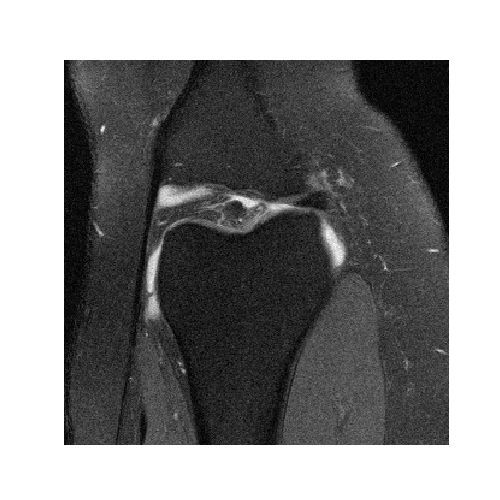
\includegraphics[width=0.1\textwidth,trim=3.3em 3.3em 3.3em 3.3em,clip]{Figures/dl_mri_figures/gt_knee.png} \textbf{image}};
        \draw [color=blue!87](image.south) |- ([xshift=-0.3ex,color=blue]exp_image.south east);
        % For kspace
        \onslide<1>{
            \path (kspace.south) ++ (0,-5em) node[anchor=south east,color=amber!87] (exp_kspace){
                \textbf{kspace} 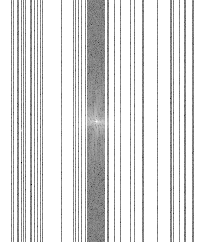
\includegraphics[width=0.1\textwidth]{Figures/intro_figures/kspace_mri.png} };
            \draw [color=amber!87](kspace.south) |- ([xshift=-0.3ex,color=amber]exp_kspace.south west);

        }
        % For aliased image
        \onslide<2>{
        \path (kspace.south) ++ (0, -4.3em) node[anchor=south east,color=amber!87] (exp_aliased_image){
            \textbf{aliased image} \includegraphics[width=0.1\textwidth,trim=3.3em 3.3em 3.3em 3.3em,clip]{Figures/dl_mri_figures/zfilled_recon_af4.png}};
        \draw [color=amber!87](kspace.south) |- ([xshift=-0.3ex,color=amber]exp_aliased_image.south west);
        }
    \end{tikzpicture}

\end{frame}

\begin{frame}{Unrolled models - 1}
    % recovery algorithm and corresponding computation graph
    % show on second slice unrolled computation graph
    We can mix the 2 single domain approaches, using the principled \textbf{optimization algorithm unrolling} method.\footfullcite{Gregor2010}

    \alt<5->{\vphantom{A graph representation of ISTA:}}{A graph representation of ISTA:}
    \begin{columns}[totalwidth=\textwidth]
        \begin{column}[]{0.3\textwidth}

            \begin{equation*}
                \begin{split}
                    \xb_{n+1} &= \highlight{yellow}{$\xb_n - \epsilon_n \mathcal{A}^H\left(\mathcal{A} \xb_n - \ybb\right)$}\\
                    \xb_{n+1} &= \alt<5->{\highlight{blue}{$f_{\thetab_n}\left(\xb_{n+1}\right)$}}{\highlight{blue}{$\tikzmarknode{prox}{\operatorname{prox}}_{\epsilon_n \mathcal{R}}\left(\xb_{n+1}\right)$}}
                \end{split}
            \end{equation*}
            \only<1>{
                \begin{tikzpicture}[overlay,remember picture,>=stealth,nodes={align=left,inner ysep=1pt},<-]
                    % For "prox"
                    \path (prox.south) ++ (0,-2.5em) node[anchor=south west,color=black!87] (exp_prox){
                        Proximity operator
                    };
                    \draw [color=black!87](prox.south) |- ([xshift=-0.3ex,color=black]exp_prox.south east);
                \end{tikzpicture}
            }

        \end{column}
        \begin{column}[]{0.6\textwidth}
            \only<1>{
                \begin{equation*}
                    \argmin_{\xb \in \mathbb{C}^n} \frac12 \|\mathcal{A} \xb - \yb \|_2^2  + \mathcal{R}(\xb)
                \end{equation*}
            }
            \only<2-3>{
                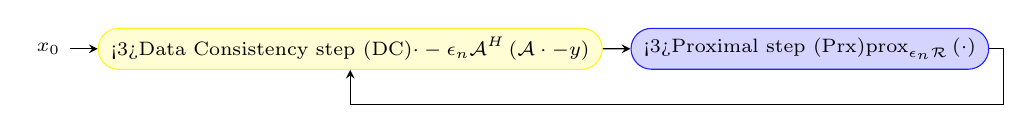
\begin{tikzpicture}[font=\scriptsize, node distance=1em,>=stealth]
                    % nodes
                    \node (input) {$\xb_0$};
                    \node (dc) [rounded rectangle, right=of input, draw=yellow!87, fill=yellow!17] {
                    \alt<3>{Data Consistency step~(DC)}{$\cdot - \epsilon_n \mathcal{A}^H\left(\mathcal{A} \cdot - \ybb\right)$}
                    };
                    \node (prox) [rounded rectangle, right=of dc, draw=blue!87, fill=blue!17] {
                        \alt<3>{Proximal step~(Prx)}{$\operatorname{prox}_{\epsilon_n \mathcal{R}}\left(\cdot\right)$}
                    };
                    % arrows linking all 4 nodes
                    \draw [->] (input) -- (dc);
                    \draw [->] (dc) -- (prox);
                    % arrow linking the prox to the dc in a loop fashion
                    \draw [->] (prox.east) -| ($(prox.east)+(0.5em, -2em)$) -| (dc.south);
                \end{tikzpicture}
            }
            \only<4->{
                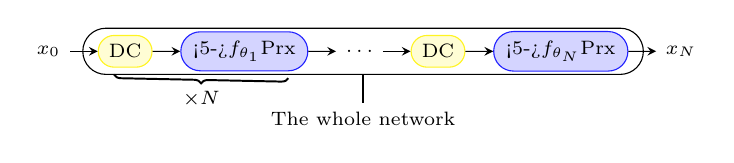
\begin{tikzpicture}[font=\scriptsize, node distance=1em,>=stealth]
                    \tikzset{
                        position label/.style={
                        below = 0.em,
                        text height = 1.5ex,
                        text depth = 1ex
                        },
                        brace/.style={
                            decoration={brace, mirror},
                            decorate
                        }
                    }
                    % nodes
                    \node (input) {$\xb_0$};
                    \node (dc_1) [rounded rectangle, right=of input, draw=yellow!87, fill=yellow!17] {DC};
                    \node (prox_1) [rounded rectangle, right=of dc_1, draw=blue!87, fill=blue!17] {\alt<5->{$f_{\thetab_1}$}{Prx}};
                    \node (dots) [right=of prox_1] {$\ldots$};
                    \node (dc_2) [rounded rectangle, right=of dots, draw=yellow!87, fill=yellow!17] {DC};
                    \node (prox_2) [rounded rectangle, right=of dc_2, draw=blue!87, fill=blue!17] {\alt<5->{$f_{\thetab_N}$}{Prx}};
                    \node (output) [right=of prox_2] {$\xb_{N}$};
                    \node (whole) [visible on=<6->, fit=(dc_1) (prox_1) (dots) (dc_2) (prox_2), draw, rounded rectangle, inner sep=0.1em] {};
                    \node (whole_exp) [visible on=<6->, below=of whole] {The whole network};
                    % arrows linking all nodes
                    \draw [->] (input) -- (dc_1);
                    \draw [->] (dc_1) -- (prox_1);
                    \draw [->] (prox_1) -- (dots);
                    \draw [->] (dots) -- (dc_2);
                    \draw [->] (dc_2) -- (prox_2);
                    \draw [->] (prox_2) -- (output);
                    % brace
                    \draw<4-5> [brace, line width=0.25mm] ($(dc_1.south west)+(0,-0.25em)$) -- ($(prox_1.south east)+(0,-0.25em)$) node [position label, pos=0.5] {$\times N$};
                    \draw<6-> [line width=0.1em] (whole.south) -- (whole_exp.north);
                \end{tikzpicture}
            }
        \end{column}
    \end{columns}
\end{frame}


\begin{frame}{Unrolled models - 2}
    % first benchmark: different unrolling strategies give different results
    \begin{exampleblock}{Contribution \#1}
        \fullcite{Ramzi2020_benchmark_journal}
    \end{exampleblock}
    % We can build different models depending on the optimization algorithm we unroll, the choice of $f_{\thetab}$ and the number of iterations.
    Different models based on:
    \begin{itemize}
        \item optimization algorithm to unroll
        \item choice of $f_{\thetab}$
        \item $N$
    \end{itemize}
    \pause

    \begin{overprint}


    \onslide<2>
        \vspace{-1em}
        \begin{table}[h]
            % \large
            \centering
            \caption{\textbf{Quantitative results for the fastMRI dataset.} The PSNR is computed over the 200 validation volumes.}
            \label{tab:quanti-fastmri}
            \vspace{-0.5em}
            \begin{tabular}{l|c|c|c|c|c}
            \textbf{Network} & \textbf{Zero-filled} & \textbf{KIKI-net} & \textbf{U-net} & \textbf{Cascade net} & \textbf{PD-net}\footnotemark \\ \hline
            \textbf{PSNR} & 29.61 & 31.38 & 31.78 & 31.97 & \textbf{32.15}
            \end{tabular}%
            \end{table}

        % XXX dk why I need to write the number manually but this needs to change
        % if the footnotes change
        \footnotetext{$^8$\fullcite{Adler2018}}
\end{overprint}



\end{frame}

\begin{frame}
    \def\thefigdim{.205}
    \def\qualifigsep{-6mm}
    \begin{figure}
        \begin{center}\hspace*{-.3cm}
        \begin{tabular}{@{\hspace*{\qualifigsep}}c@{\hspace*{\qualifigsep}}c@{\hspace*{\qualifigsep}}c@{\hspace*{\qualifigsep}}c@{\hspace*{\qualifigsep}}c@{\hspace*{\qualifigsep}}c@{\hspace*{\qualifigsep}}}
        {\textbf{Reference}} & {\textbf{Zero-filled}} & {\textbf{KIKI-net}} & {\textbf{U-net}} & {\textbf{Cascade-net}} & {\textbf{PD-net}} \\
        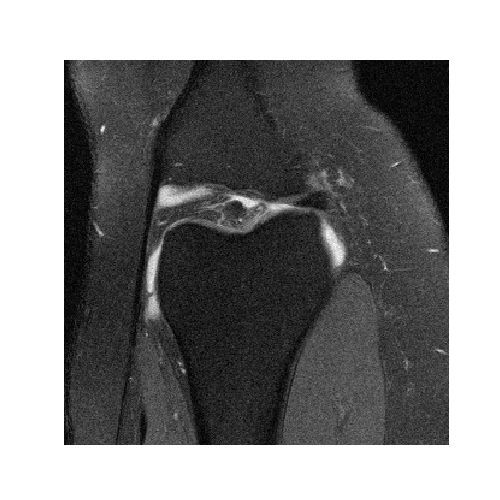
\includegraphics[width=\thefigdim\linewidth]{Figures/dl_mri_figures/bench_figs/image_gt.png}&
        \includegraphics[width=\thefigdim\linewidth]{Figures/dl_mri_figures/bench_figs/zfilled_recon_af4.png}&
        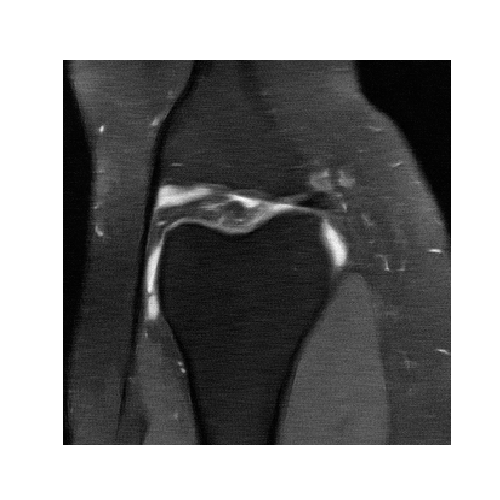
\includegraphics[width=\thefigdim\linewidth]{Figures/dl_mri_figures/bench_figs/kikinet-sep-16_recon_af4.png}&
        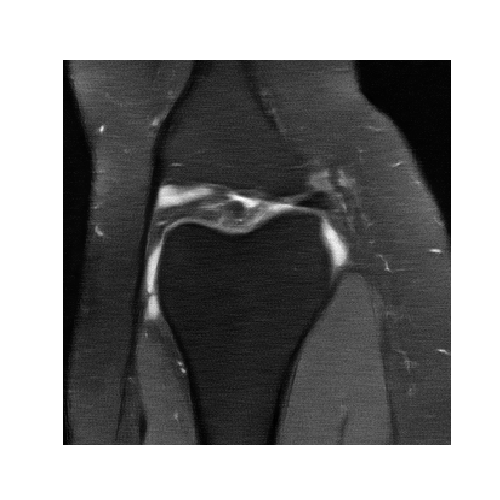
\includegraphics[width=\thefigdim\linewidth]{Figures/dl_mri_figures/bench_figs/unet_recon_af4.png}&
        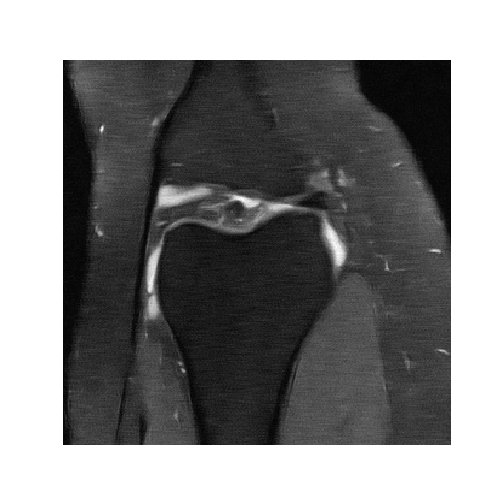
\includegraphics[width=\thefigdim\linewidth]{Figures/dl_mri_figures/bench_figs/cascadenet_recon_af4.png}&
        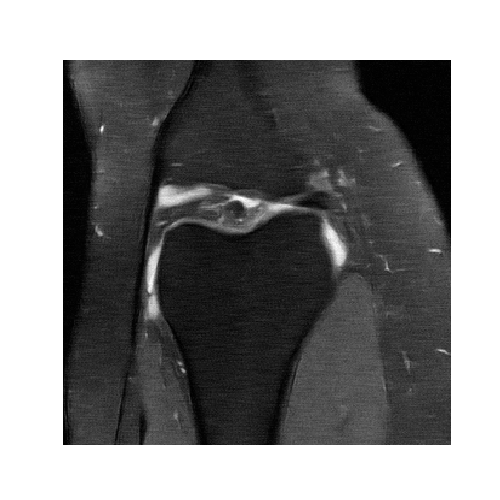
\includegraphics[width=\thefigdim\linewidth]{Figures/dl_mri_figures/bench_figs/pdnet_recon_af4.png}\\[-.70cm]
        &
        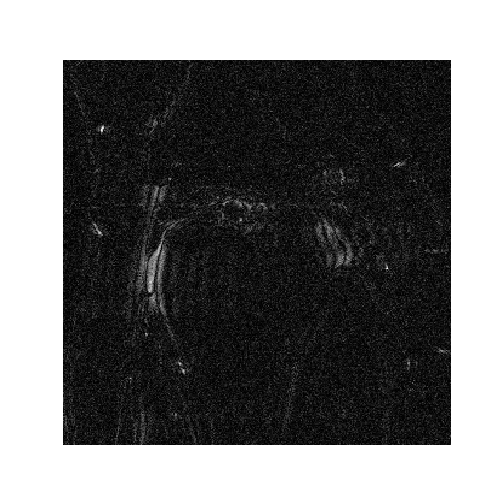
\includegraphics[width=\thefigdim\linewidth]{Figures/dl_mri_figures/bench_figs/zfilled_residu_af4.png}&
        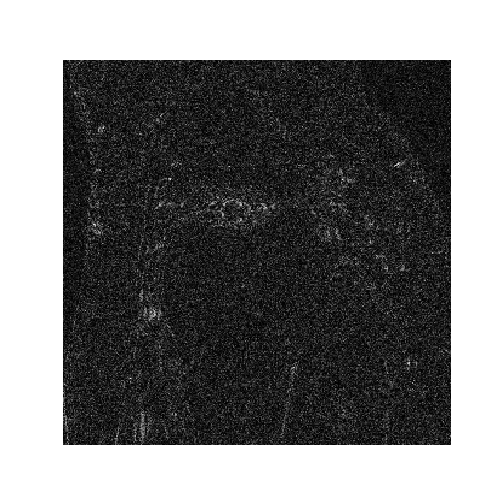
\includegraphics[width=\thefigdim\linewidth]{Figures/dl_mri_figures/bench_figs/kikinet-sep-16_residu_af4.png}&
        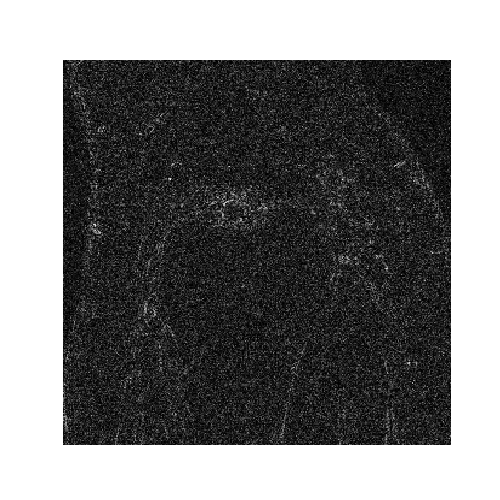
\includegraphics[width=\thefigdim\linewidth]{Figures/dl_mri_figures/bench_figs/unet_residu_af4.png}&
        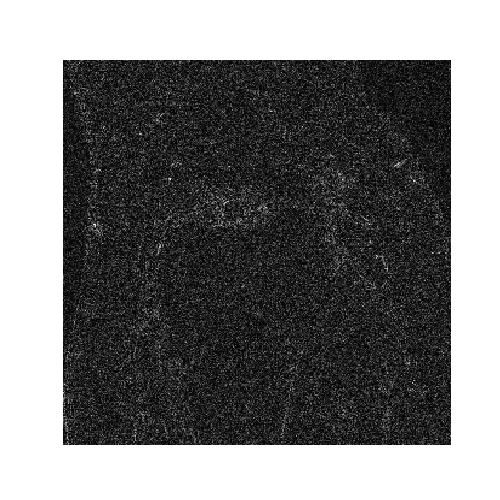
\includegraphics[width=\thefigdim\linewidth]{Figures/dl_mri_figures/bench_figs/cascadenet_residu_af4.png}&
        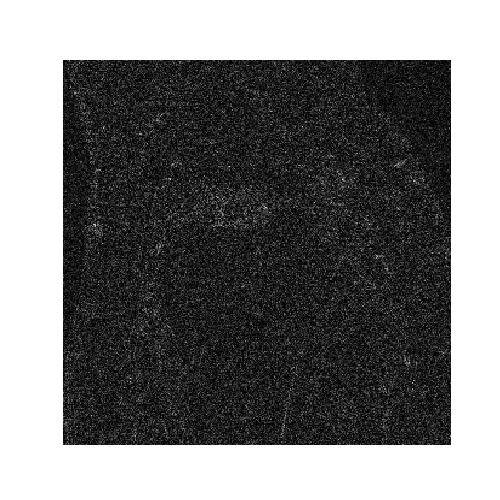
\includegraphics[width=\thefigdim\linewidth]{Figures/dl_mri_figures/bench_figs/pdnet_residu_af4.png}
        \end{tabular}
        \end{center}
        \end{figure}
\end{frame}


\begin{frame}{Unrolled models - 2}
    % first benchmark: different unrolling strategies give different results
    \begin{exampleblock}{Contribution \#1}
        \fullcite{Ramzi2020_benchmark_journal}
    \end{exampleblock}
    % We can build different models depending on the optimization algorithm we unroll, the choice of $f_{\thetab}$ and the number of iterations.
    Different models based on:
    \begin{itemize}
        \item optimization algorithm to unroll
        \item choice of $f_{\thetab}$
        \item $N$
    \end{itemize}


    \noindent\rule{\textwidth}{1pt}

        \begin{itemize}
            \item \faicon{github} Code available online: \texttt{github.com/zaccharieramzi/fastmri-reproducible-benchmark}
            \item\begin{tabular}{@{}c@{}}
\includegraphics[width=3ex]{Figures/hf_logo.jpeg}\end{tabular}Model weights available online: \texttt{huggingface.co/zaccharieramzi}
        \end{itemize}



\end{frame}

\begin{frame}{XPDNet}

\end{frame}

\begin{frame}{XPDNet}
    % talk about XPDNet archi
    \begin{center}
        \begin{tikzpicture}[
            font=\Large, node distance=1.5em,>=stealth,
            ionode/.style={rounded rectangle, draw=red!87, fill=red!17},
            unitnode/.style={rounded rectangle, draw=black!87, fill=black!7},
            opnode/.style={rounded rectangle, draw=green!87, fill=green!17},
            kspace_node/.style={rounded rectangle, draw=yellow!87, fill=yellow!17},
            image_node/.style={rounded rectangle, draw=blue!87, fill=blue!17},
            highlight_node/.style={rectangle, draw=red!70, dashed, inner sep=0.1em},
        ]
            % Unrolled net simple
            \node (input) {$\xb_0$};
            \only<1-2>{
                % nodes
                \node (first_unit) [fit=(dc_1)(prox_1), unitnode, inner sep=0.7em, visible on=<2>] {};
                \node (t_first_unit) [below right, visible on=<2>] at ($(first_unit.north west)+(-0.9em,0.25em)$) {\tiny Iteration Unit~(IU)};
                \node (second_unit) [fit=(dc_2)(prox_2), unitnode, inner sep=0.5em, visible on=<2>] {};
                \node (input) {$\xb_0$};
                \node (dc_1) [right=of input, kspace_node] {DC};
                \node (prox_1) [right=of dc_1, image_node] {$f_{\thetab_1}$};
                \node (dots) [right=of prox_1] {$\ldots$};
                \node (dc_2) [right=of dots, kspace_node] {DC};
                \node (prox_2) [right=of dc_2, image_node] {$f_{\thetab_N}$};
                \node (output) [right=of prox_2] {$\xb_{N}$};
                % arrows linking all nodes
                \draw [->] (input) -- (dc_1);
                \draw [->] (dc_1) -- (prox_1);
                \draw [->] (prox_1) -- (dots);
                \draw [->] (dots) -- (dc_2);
                \draw [->] (dc_2) -- (prox_2);
                \draw [->] (prox_2) -- (output);
            }
            % Unrolled net exploded
            \only<3->{
                % nodes
                %% main track
                \node (first_unit) [unitnode, right=of input] {IU};
                \node (dots) [right=of first_unit] {$\ldots$};
                \node (second_unit) [unitnode, right=of dots] {IU};
                \node (output) [right=of second_unit] {$\xb_{N}$};
                %% IU track
                %% applies \mathcal{A} (in green), then removes \ybb (in yellow), then applies \epsilon_1 \mathcal{A}^H (in green)
                %% then residual connection , then applies f_{\thetab_1} (in blue)
                \node (forward_op) [opnode, below=4em of first_unit] {$\mathcal{A} \cdot$};
                \node (input_forward) [left=3em of forward_op] {};
                \node (input_str_forward) [left=of input_forward] {$\xb_0$};
                \node (dc) [kspace_node, above right=of forward_op] {$\cdot - \ybb$};
                \node (backward_op) [opnode, right=of dc, visible on=<3>] {$\epsilon_1 \mathcal{A}^H \cdot$};
                \node (simple_backward_op) [opnode, right=of dc, visible on=<4->] {$\mathcal{A}^H \cdot$};
                \node (dc_res) [rounded rectangle, draw, fill=white, below right=of backward_op, visible on=<3>] {$-$};
                \node (dc_concat) [rounded rectangle, draw, fill=white, below right=of backward_op, visible on=<4->] {$\operatorname{concat}$};
                \node (prox) [image_node, right=of dc_concat] {$f_{\thetab_1}$};
                \node (prox_exp_cnn) [below=2em of prox, visible on=<3-4>] {CNN};
                \node (prox_exp_mwcnn) [below=2em of prox, visible on=<5->] {MWCNN\footfullcite{Liu2018}};
                \node (outpt_prox) [right=3em of prox] {$\xb_1$};
                % smaps nodes
                \node (smaps_refiner) [opnode, below left=of forward_op, visible on=<6->] {Smaps refiner\footfullcite{Sriram2020End-to-EndReconstruction}};
                \node (smaps) [left=of smaps_refiner, visible on=<6->] {$\Sbb$};
                \node (smaps_exp) [below=0.4em of smaps_refiner, visible on=<6->] {U-Net\footfullcite{ronneberger2015u}};
                \begin{scope}[on background layer]
                    \node (encompassing_unit) [unitnode, fit=(forward_op)(dc)(simple_backward_op)(backward_op)(dc_concat)(dc_res)(prox), inner sep=0.9em] {};
                    %% highlighting nodes
                    \node (highlight_concat) [highlight_node, fit=(backward_op) (dc_concat), visible on=<4>] {};
                    \node (highlight_mwcnn) [highlight_node, fit=(prox_exp_mwcnn), visible on=<5>] {};
                    \node (highlight_smaps) [highlight_node, fit=(smaps_refiner) (smaps) (smaps_exp), visible on=<6>] {};
                \end{scope}
                % arrows linking all nodes
                %% main track
                \draw [->] (input) -- (first_unit);
                \draw [->] (first_unit) -- (dots);
                \draw [->] (dots) -- (second_unit);
                \draw [->] (second_unit) -- (output);
                %% IU track
                \draw [->] (input_forward) -- (forward_op);
                \draw [->] (forward_op) -| (dc);
                \draw<3> [->] (dc) -- (backward_op);
                \draw<4-> [->] (dc) -- (simple_backward_op);
                \draw<3> [->] (backward_op) -| (dc_res);
                \draw<4-> [->] (simple_backward_op) -| (dc_concat);
                \draw<3> [->] plot [smooth, tension=0.7] coordinates{(input_forward.east)  ($(forward_op.south)+(0, -0.6em)$) (dc_res.west)};
                \draw<4-> [->] plot [smooth, tension=0.7] coordinates{(input_forward.east)  ($(forward_op.south)+(0, -0.6em)$) (dc_concat.west)};
                \draw (input_str_forward) -- (input_forward.east);
                \draw<3> [->] (dc_res) -- (prox);
                \draw<4-> [->] (dc_concat) -- (prox);
                \draw [->] (prox) -- (outpt_prox);
                \draw [line width=0.1em] (first_unit.south) -- (encompassing_unit.north west);
                \draw<3-4> [line width=0.1em] (prox.south) -- (prox_exp_cnn.north);
                \draw<5-> [line width=0.1em] (prox.south) -- (prox_exp_mwcnn.north);
                % smaps arrows
                \draw<6-> [<-] (smaps_refiner) -- (smaps);
                \draw<6-> [->] (smaps_refiner) -| (forward_op);
                \draw<6-> [->] (smaps_refiner) -| (simple_backward_op);
                \draw<6-> [line width=0.1em] (smaps_refiner.south) -- (smaps_exp.north);
            }

        \end{tikzpicture}
    \end{center}
\end{frame}

\begin{frame}{fastMRI challenge}
    % mention fastMRI challenge results
    \begin{exampleblock}{Contributions \#2}
        \begin{itemize}
            \item \fullcite{Muckley2021}
            \item \fullcite{Ramzi2020_xpdnet}
        \end{itemize}
    \end{exampleblock}

    \begin{overprint}

        \onslide<2>
        \noindent\rule{\textwidth}{1pt}

        \begin{itemize}
            \item Data: fastMRI
            \item Compute: Jean Zay
        \end{itemize}

        \onslide<3>
        \begin{table}[]
            \centering
            \caption{\textbf{fastMRI challenge radiologist evaluation.}}
            \label{tab:fastmri-challenge}
            \begin{tabular}{|l|c|c|}
            \hline
            \textbf{Team}      & \textbf{Rank 4X} & \textbf{Rank 8X} \\ \hline
            \textbf{AIRS}      & 1.36             & 1.28             \\ \hline
            \highlight{blue}{\textbf{NeuroSpin}} & 1.94             & 2.25             \\ \hline
            \textbf{ATB}       & 2.22             & 2.28             \\ \hline
            \end{tabular}
        \end{table}
    \end{overprint}
\end{frame}


\begin{frame}
    \def\thefigdimigogd{.35}

    \hspace*{-.7cm}
    \begin{tabular}{c@{\hspace*{\qualifigsepigogd}}c@{\hspace*{\qualifigsepigogd}}c}
        {\textbf{Reference}} & \makecell{{\textbf{GRAPPA }} \\ PSNR: 26, SSIM: 0.77} & \makecell{{\textbf{XPDNet}} \\ PSNR: 36, SSIM: 0.96} \\
        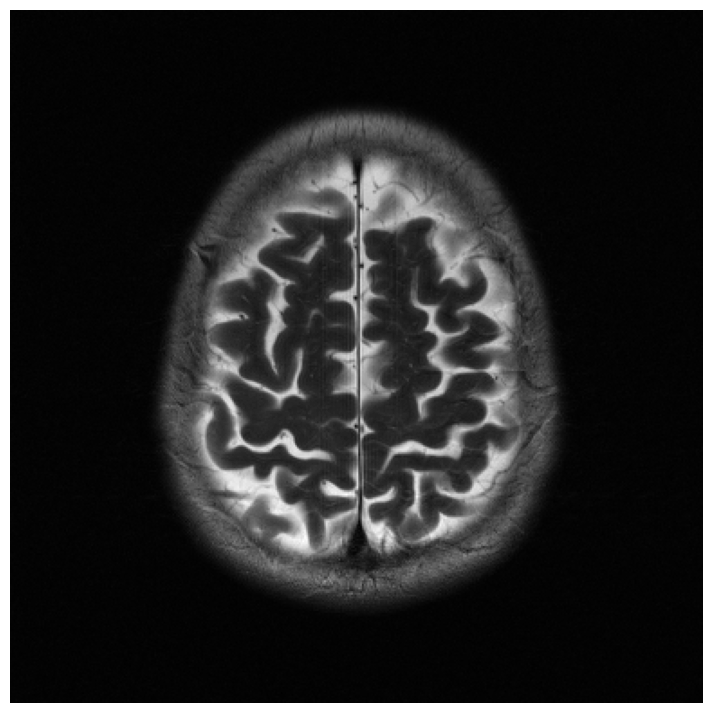
\includegraphics[width=\thefigdimigogd\textwidth]{Figures/clinic_applic/fastmri_r8/GT_Pinf_S1.0000.png}&
        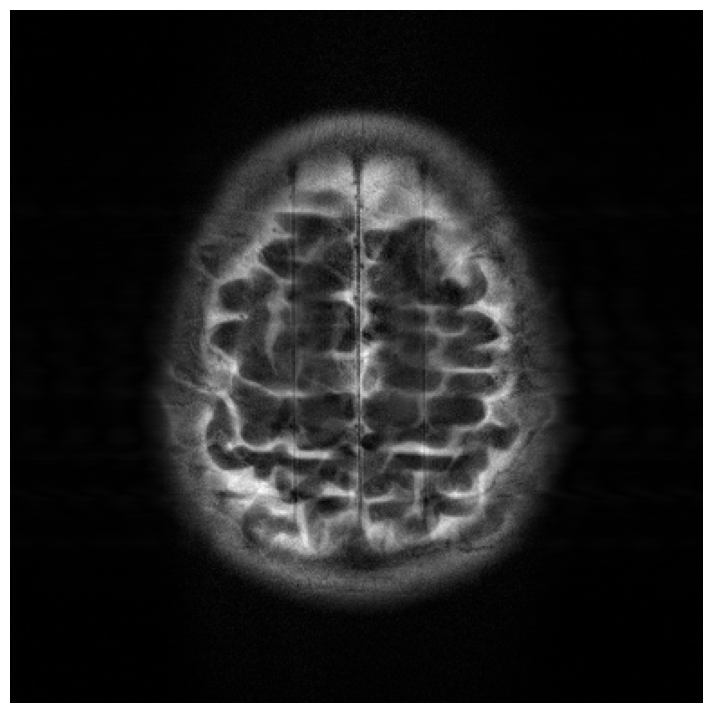
\includegraphics[width=\thefigdimigogd\textwidth]{Figures/clinic_applic/fastmri_r8/GRAPPA-ideal_P26.18_S0.7704.png}&
        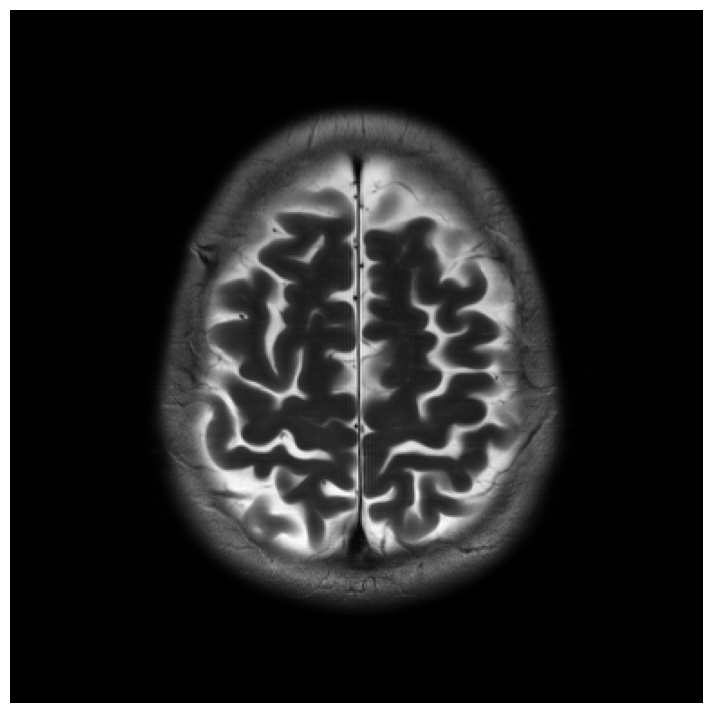
\includegraphics[width=\thefigdimigogd\textwidth]{Figures/clinic_applic/fastmri_r8/NN_P36.82_S0.9626.png}
    \end{tabular}

\end{frame}

\begin{frame}{Robustness test}
    % XXX: only if we decide not to have clinical applicability
    % How does the XPDNet fare in a prospective out-of-distribution setting:
    XPDNet in a prospective out-of-distribution setting:\footfullcite{Marrakchi-Kacem2016RobustChoices}

    different orientation, higher resolution, higher field strength, lower acceleration factor, presence of the cerebellum.\footnote{For anonymity reasons, the cerebellum is not present in the fastMRI dataset.}

\end{frame}

\begin{frame}
    \begin{figure}[h]
        \begin{center}
        \begin{tabular}{c@{\hspace*{\qualifigsepigogd}}c}
        {\textbf{GRAPPA }} & {\textbf{XPDNet}} \\
        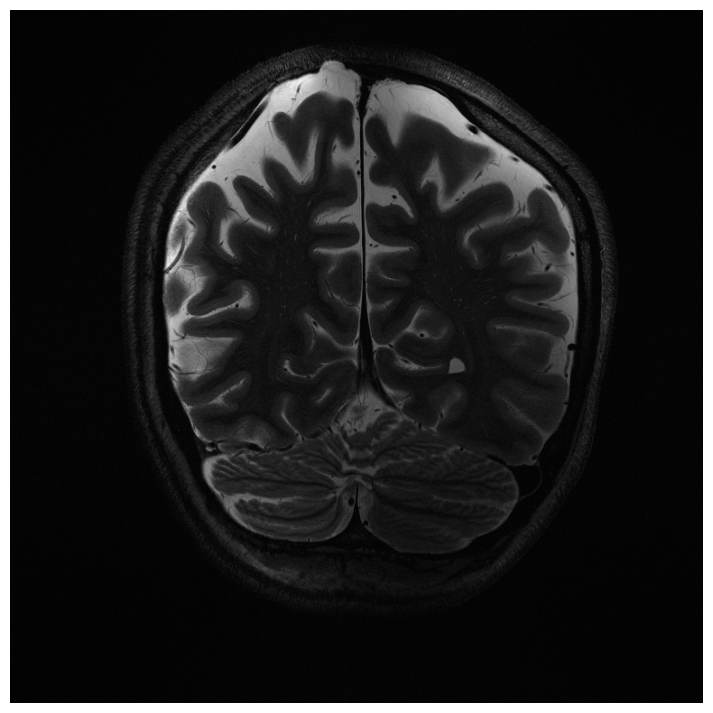
\includegraphics[width=0.38\textwidth]{Figures/clinic_applic/gt_brain_7t.png}&
        \includegraphics[width=0.38\textwidth]{Figures/clinic_applic/brain_nn_recon.png}\\
        \includegraphics[width=0.38\textwidth]{Figures/clinic_applic/gt_brain_7t_zoom.png}&
        \includegraphics[width=0.38\textwidth]{Figures/clinic_applic/brain_nn_recon_zoom.png}
        \end{tabular}
        \caption{\textbf{XPDNet reconstruction on a brain prospectively accelerated.} (zoom on the cerebellum) \label{fig:brain-7t}}
        \end{center}
        \end{figure}
\end{frame}

\begin{frame}{Non-Cartesian acquisitions}
    % Why do we need non-Cartesian acquisitions?
    % We need non-Cartesian acquisitions to better cover the k-space.
    Non-Cartesian acquisitions better cover the k-space.
    \pause
    \vspace{-1ex}
    \begin{figure}
        \centering
        \begin{subfigure}{0.48\textwidth}
            \includegraphics[height=0.48\textheight]{Figures/dl_mri_figures/radial_trajectory.png}
        \end{subfigure}
        \begin{subfigure}{0.48\textwidth}
            \includegraphics[height=0.48\textheight]{Figures/dl_mri_figures/spiral_trajectory.png}
        \end{subfigure}
        \caption{\textbf{Radial and spiral undersampled trajectories.}}
    \end{figure}
    \pause

    % The difficulty from a computational point of view is that we need to now use the \textbf{Nonuniform Fourier Transform (NDFT)}.
    \textbf{Nonuniform Fourier Transform (NDFT)} too costly $\Rightarrow$ NUFFT, with the TensorFlow implementation:
    % We resort to using its fast approximation, the NUFFT, which we implemented in TensorFlow, to enable gradient-based learning:
    \begin{itemize}
        \item \faicon{github} Code available online: \texttt{github.com/zaccharieramzi/tfkbnufft}
    \end{itemize}
\end{frame}

\begin{frame}{NC-PDNet - 1}
    % explain NC-PDNet and density compensation
    \begin{center}
        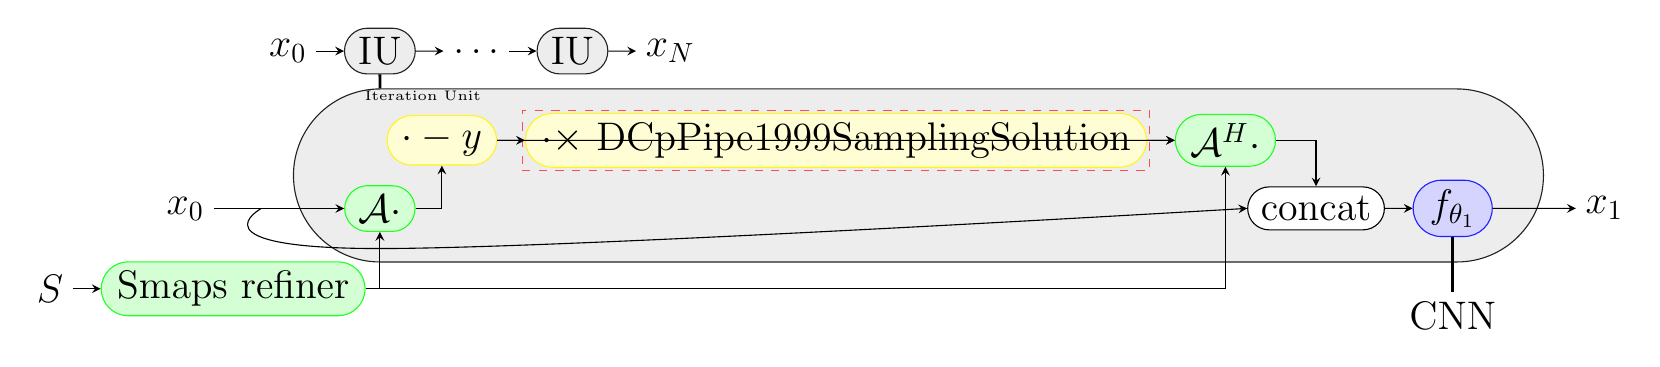
\begin{tikzpicture}[
            font=\Large, node distance=1em,>=stealth,
            ionode/.style={rounded rectangle, draw=red!87, fill=red!17},
            unitnode/.style={rounded rectangle, draw=black!87, fill=black!7},
            opnode/.style={rounded rectangle, draw=green!87, fill=green!17},
            kspace_node/.style={rounded rectangle, draw=yellow!87, fill=yellow!17},
            image_node/.style={rounded rectangle, draw=blue!87, fill=blue!17},
            highlight_node/.style={rectangle, draw=red!70, dashed, inner sep=0.1em},
        ]
            % Unrolled net simple
            \node (input) {$\xb_0$};
            % Unrolled net exploded
            % nodes
            %% main track
            \node (first_unit) [unitnode, right=of input] {IU};
            \node (dots) [right=of first_unit] {$\ldots$};
            \node (second_unit) [unitnode, right=of dots] {IU};
            \node (output) [right=of second_unit] {$\xb_{N}$};
            %% IU track
            %% applies \mathcal{A} (in green), then removes \ybb (in yellow), then applies \epsilon_1 \mathcal{A}^H (in green)
            %% then residual connection , then applies f_{\thetab_1} (in blue)
            \node (forward_op) [opnode, below=4em of first_unit] {$\mathcal{A} \cdot$};
            \node (input_forward) [left=3em of forward_op] {};
            \node (input_str_forward) [left=of input_forward] {$\xb_0$};
            \node (dc) [kspace_node, above right=of forward_op] {$\cdot - \ybb$};
            \node (dcp) [kspace_node, right=of dc, visible on=<2->] {$\cdot \times$ DCp\footfullcite{Pipe1999SamplingSolution}};
            \node (backward_op) [opnode, right=of dcp] {$\mathcal{A}^H \cdot$};
            \node (dc_input_comb) [rounded rectangle, draw, fill=white, below right=of backward_op] {$\operatorname{concat}$};
            \node (prox) [image_node, right=of dc_input_comb] {$f_{\thetab_1}$};
            \node (prox_exp) [below=2em of prox] {CNN};
            \node (outpt_prox) [right=3em of prox] {$\xb_1$};
            \begin{scope}[on background layer]
                \node (encompassing_unit) [unitnode, fit=(forward_op)(dc)(backward_op)(dc_input_comb)(prox), inner sep=0.9em] {};
                \node (t_first_unit) [below right] at ($(encompassing_unit.north west)+(-0.9em,0.25em)$) {\tiny Iteration Unit};
            \end{scope}
            %% smaps nodes
            \node (smaps_refiner) [opnode, below left=1.5em of forward_op] {Smaps refiner};
            \node (smaps) [left=of smaps_refiner] {$\Sbb$};
            %% highlight nodes
            \node<2> (highlight_dcp) [highlight_node, fit=(dcp)] {};
            % arrows linking all nodes
            %% main track
            \draw [->] (input) -- (first_unit);
            \draw [->] (first_unit) -- (dots);
            \draw [->] (dots) -- (second_unit);
            \draw [->] (second_unit) -- (output);
            %% IU track
            \draw [->] (input_forward) -- (forward_op);
            \draw [->] (forward_op) -| (dc);
            \draw<2-> [->] (dc) -- (dcp);
            \draw<2-> [->] (dcp) -- (backward_op);
            \draw<1> [->] (dc) -- (backward_op);
            \draw [->] (backward_op) -| (dc_input_comb);
            \draw [->] plot [smooth, tension=0.7] coordinates{(input_forward.east) ($(forward_op.south)+(0, -0.6em)$) (dc_input_comb.west)};
            \draw (input_str_forward) -- (input_forward.east);
            \draw [->] (dc_input_comb) -- (prox);
            \draw [->] (prox) -- (outpt_prox);
            \draw [line width=0.1em] (first_unit.south) -- (encompassing_unit.north west);
            \draw [line width=0.1em] (prox.south) -- (prox_exp.north);
            % smaps arrows
            \draw [<-] (smaps_refiner) -- (smaps);
            \draw [->] (smaps_refiner) -| (forward_op);
            \draw [->] (smaps_refiner) -| (backward_op);

        \end{tikzpicture}
    \end{center}
\end{frame}

\begin{frame}{NC-PDNet - 2}
    % give results
    \begin{exampleblock}{Contribution \#3}
        \fullcite{Ramzi2021_ncpdnet_journal}
    \end{exampleblock}


\end{frame}

\begin{frame}
    \begin{figure}
        \begin{overprint}
            \onslide<1>\centering\includegraphics[height=0.9\textheight]{Figures/dl_mri_figures/single_coil.pdf}\caption{\textbf{2D single-coil reconstruction quantitative results on the fastMRI knee dataset.}}
            \onslide<2>\centering\includegraphics[width=\textwidth]{Figures/dl_mri_figures/quali_no_err_af4_radial.pdf}\caption{\textbf{2D single-coil reconstruction qualitative results on the fastMRI dataset for a radial trajectory.}}
            \onslide<3>\centering\includegraphics[width=0.7\textwidth]{Figures/dl_mri_figures/3d.pdf}\caption{\textbf{3D single-coil reconstruction quantitative results on the OASIS dataset for a radial trajectory.}}
            \onslide<4>\centering\includegraphics[width=\textwidth]{Figures/dl_mri_figures/quali_no_err_3d_af4_radial.pdf}\caption{\textbf{3D single-coil reconstruction qualitative results on the OASIS dataset for a radial trajectory.}}
        \end{overprint}
    \end{figure}
\end{frame}

\begin{frame}{Unrolled models for MRI reconstruction}
    % cool: we are starting to have good results, let's not forget the end goal
    % use this in a scanner so that the MRI exam is faster
    % how will this technique fare in the clinical setting ? <This would be in the case of using clinical applic chapther>
    % <otherwise>: ok we get good results, but we have sacrificed a bit of power in 3D, and multi-coil is not possible as is
    \begin{block}{Recap}
        MRI is slow because of \textbf{relaxation}.

        \pause
        If we want to do fewer relaxations, we need to exploit some \textbf{redundancy} in MR images.

        \pause
        \textbf{Deep Learning} allows us to learn more complex structures in MR images than Compressed Sensing.
        We showcased 2 instances of unrolled models, \textbf{XPDNet} and \textbf{NC-PDNet}, which can perform really well in challenging acquisition settings.
    \end{block}

    \pause
    But we needed to trade off some model capacity for memory, in order to train the models in the 3D single-coil case.
    How will this fare going to 3D multi-coil?
\end{frame}

% \section{Clinical applicability}

\begin{frame}[plain,c]
    %\frametitle{A first slide}

    \begin{center}
        \color{DarkBlue}
    \Huge \thesection. \insertsection
    \end{center}

\end{frame}


\begin{frame}{Learnlets - 1}
    % show the generalization figure
    \begin{figure}
        \centering
        \includegraphics[height=0.8\textheight]{Figures/clinic_applic/learnlets_tikz_reduced.pdf}
    \end{figure}
\end{frame}

\begin{frame}{Learnlets - 2}
    % show the generalization figure
    \begin{figure}[ht]
        \includegraphics[height=0.78\textheight]{Figures/clinic_applic/model_comparison.pdf}
        \caption{\textbf{Denoising performance.}}
        \end{figure}
\end{frame}

\begin{frame}{Denoising Score Matching - 1}
    % show the samples
    Optimal denoiser:\footfullcite{Vincent2011,Alain2013}
    \begin{equation*}
        \rb^\star(\xb', \sigma) = \xb' + \sigma^2 \nabla_{\xb} \log p_{\sigma^2}(\xb')
    \end{equation*}
    where $p_{\sigma^2} = p \ast \mathcal{N}(0, \sigma^2)$.
\end{frame}

\begin{frame}{Denoising Score Matching - 2}
    % show the samples
    \begin{figure}
        \centering
        \includegraphics[width=\textwidth]{Figures/clinic_applic/dsm_main.pdf}
    \end{figure}

\end{frame}

\section{Going even deeper}

\begin{frame}[plain,c]
    %\frametitle{A first slide}
    
    \begin{center}
        \color{DarkBlue}
    \Huge Going even deeper
    \end{center}
    
\end{frame}

\subsection{Implicit models}

\begin{frame}{Why should we go deep?}
    % with deeper models, comes better performance
    % figure of Pezzotti et al.
    The general empirical gist of DL is that with deeper models comes better performance.
    \begin{figure}
        \begin{overprint}
            \onslide<2>\centering\includegraphics[width=0.4\textwidth]{Figures/shine_figures/more_layers.jpg}\caption{Credits: \href{reddit.com/r/ProgrammerHumor/comments/5si1f0/machine_learning_approaches/}{reddit.com/r/ProgrammerHumor/comments/5si1f0/machine\_learning\_approaches/}}
            \onslide<3>\centering\includegraphics[width=0.78\textwidth]{Figures/shine_figures/pezzotti.png}\caption{\textbf{Performance of an unrolled MRI reconstruction network function of the number of iteration units (blocks).}\footfullcite{Pezzotti2020AnReconstruction}}
        \end{overprint}
    \end{figure}
\end{frame}

\begin{frame}{Can we go deeper?}
    % in the current state not: activations + constrained memory
    The big problem at hand is that deeper models need more \textbf{memory} to train, and the memory we have is constrained.
    \pause

    This memory requirement comes primarily from the \textbf{activations} of the model, not from the model weights.
    \pause

    \begin{center}
        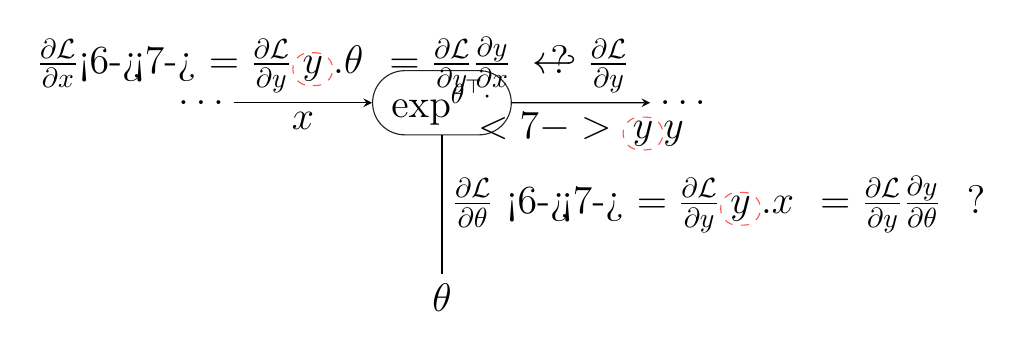
\begin{tikzpicture}[
            font=\Large, node distance=5em,>=stealth,
            highlight/.style={rounded rectangle, draw=red!67, dashed, inner sep=0.1em},
        ]
            % nodes
            \node (input) {$\ldots$};
            \node (op) [rounded rectangle, right=of input, draw=black!87] {$\exp^{\thetab^\top \cdot}$};
            \node (output) [right=of op] {$\ldots$};
            \node (op_params) [below=of op] {$\thetab$};
            % arrows
            %% input to op
            \draw[->] (input.east) -- node [midway,below] {$\xb$} node [midway,above, visible on=<5->] {
                $\frac{\partial \mathcal{L}}{\partial \xb}$\alt<6->{\hspace{-0.5em}
                    \alt<7->{
                        $= \frac{\partial \mathcal{L}}{\partial \yb} \tikzmarknode[highlight]{y_x}{\yb} . \thetab $
                    }{
                        $= \frac{\partial \mathcal{L}}{\partial \yb} \frac{\partial \yb}{\partial \xb}$
                    }
                }{ ?}
            } (op.west);
            %% op to output
            \draw[->] (op) -- node (y) [midway,below] {$\alt<7->{\tikzmarknode[highlight]{y}{\yb}}{\yb}$} node [midway,above, visible on=<4->] {$\hookleftarrow \frac{\partial \mathcal{L}}{\partial \yb}$}  (output);
            %% op to op_params
            \draw[line width=0.1em] (op.south) -- node [midway, right, visible on=<5->] {
                $\frac{\partial \mathcal{L}}{\partial \thetab}$ \alt<6->{\hspace{-0.5em}
                    \alt<7->{
                        $= \frac{\partial \mathcal{L}}{\partial \yb} \tikzmarknode[highlight]{y_theta}{\yb} . \xb $
                    }{
                        $= \frac{\partial \mathcal{L}}{\partial \yb} \frac{\partial \yb}{\partial \thetab}$
                    }
                }{?}
            } (op_params.north);
        \end{tikzpicture}    
    \end{center}
    
\end{frame}

\begin{frame}{The modeling solutions}
    % gradient checkpointing
    % Invertible networks
    % Implicit models
    On the modeling side, several solutions exist:
    \begin{itemize}[<+->]
        \item Gradient checkpointing~\citep{Chen2016TrainingCost}
        \item Invertible networks~\citep{Gomez2017TheActivations,Sander2021MomentumNetworks}
        \item Implicit models~\citep{Chen2018NeuralEquations,Bai2019DeepModels}
    \end{itemize}
\end{frame}

\begin{frame}{Deep Equilibrium networks - 1}
    % give equation and how to compute the gradient with IFT
    \citet{Bai2019DeepModels} introduced \textbf{Deep Equilibrium networks~(DEQs)}, a type of implicit model.
    The output of DEQs is defined implicitly as the solution to a fixed-point equation.

    \begin{equation*}
        h_{\thetab}(\xb) = \zb^\star, \text{ where } \alt<3>{g_\thetab(\zb^\star, \xb) = \zb^\star - f_\thetab(\zb^\star, \xb) = 0}{\zb^\star = f_\thetab(\zb^\star, \xb)}
    \end{equation*}

    \pause

    In practice, we solve this equation with a \textbf{quasi-Newton method}.
\end{frame}

\begin{frame}{Deep Equilibrium networks - 2}
    The big question is now: how do I compute the gradient $\frac{\partial \mathcal{L}}{\partial \thetab}$?
    \pause

    The \textbf{Implicit Function Theorem} gives us just that:
    \begin{theorem}[Hypergradient~\citep{Krantz2013TheApplications,Bai2019DeepModels}]
        Let $\thetab \in \mathbb{R}^p$ be a set of parameters, let $\mathcal{L}: \mathbb{R}^d \rightarrow \mathbb{R}$ be a loss function and $g_{\thetab}: \mathbb{R}^d \rightarrow \mathbb{R}^d$ be a root-defining function.
Let $\zb^\star \in  \mathbb{R}^d$ such that $g_{\thetab}(\zb^\star) = 0$ and $J_{g_{\thetab}}(\zb^\star) = \frac{\partial g_{\theta}}{\partial \zb}\Bigr|_{\zb^\star}$ is invertible, then the gradient of the loss $\mathcal{L}$ wrt. $\thetab$, called Hypergradient, is given by
\begin{equation*}
    \frac{\partial \mathcal{L}}{\partial \thetab}\Bigr|_{\zb^\star} = \nabla_\zb \mathcal{L}(\zb^\star)^\top J_{g_{\thetab}}(\zb^\star)^{-1} \frac{\partial g_{\thetab}}{\partial \thetab}\Bigr|_{\zb^\star} \, .
\end{equation*}
    \end{theorem}
    \pause

    Key for our memory problem: it does not rely on any activations you could have when solving the fixed-point equation.
\end{frame}

\subsection{SHINE}
\begin{frame}{The limits of DEQs}
    % they are slow to train
    DEQs achieve excellent results in NLP~(Natural Language Processing) and CV~(Computer Vision) tasks, but they are slow to train.

    \begin{figure}
        \centering
        \includegraphics[width=0.6\textwidth]{Figures/shine_figures/deq_memory.png}
        \caption{\textbf{Performance, memory and training speed of DEQs.}~\citep{Bai2020MultiscaleModels}}
    \end{figure}
\end{frame}

\begin{frame}{Why are DEQs slow?}
    % bc of Jacobian inversion
    If we look back the equation used to compute the gradient of DEQs:
    \begin{equation*}
        \frac{\partial \mathcal{L}}{\partial \thetab}\Bigr|_{\zb^\star} = \highlight{green}{$\nabla_\zb \mathcal{L}(\zb^\star)^\top$} \highlight{red}{$J_{g_{\thetab}}(\zb^\star)^{-1}$} \frac{\partial g_{\thetab}}{\partial \thetab}\Bigr|_{\zb^\star} \, ,
    \end{equation*}
    we see that we need to invert a huge matrix \highlight{red}{$J_{g_{\thetab}}(\zb^\star)$} in a certain direction \highlight{green}{$\nabla_\zb \mathcal{L}(\zb^\star)$}.
    \pause

    In practice this is done using an iterative algorithm.
\end{frame}

\begin{frame}{Can we avoid the Jacobian inversion?}
    % yes: reuse a by-product of the forward pass, share the inverse estimate
    \begin{exampleblock}{Contribution}
        \fullcite{Ramzi2021_shine}
    \end{exampleblock}
    
    We introduced \textbf{SHINE: SHaring the INverse Estimate}.

    \begin{equation*}
        \tikzmarknode{qn_matrix}{\highlight{blue}{$\Bb^{-1}$}} \approx \tikzmarknode{true_jacobian}{\highlight{red}{$J_{g_{\thetab}}(\zb^\star)^{-1}$}}
    \end{equation*}

    \begin{tikzpicture}[overlay,remember picture,>=stealth,nodes={align=left,inner ysep=1pt},<-]
        % For "kspace"
        \onslide<2->{
        \path (true_jacobian.south) ++ (0,-2em) node[anchor=south west,color=red!87] (exp_jac){
            \textbf{True Jacobian inverse}};
        \draw [color=red!87](true_jacobian.south) |- ([xshift=-0.3ex,color=red]exp_jac.south east);
        }
        % For "image"
        \onslide<3->{
        \path (qn_matrix.south) ++ (0, -2em) node[anchor=south east,color=blue!87] (exp_qnm){
            \textbf{quasi-Newton matrix}};
        \draw [color=blue!87](qn_matrix.south) |- ([xshift=-0.3ex,color=blue]exp_qnm.south west);
    }
    \end{tikzpicture}
    \pause
    \onslide<4->

    \hfill \break
    Properties of \highlight{blue}{$\Bb$}:
    \begin{itemize}
        \item<4-> It is computed when solving $g_\thetab(\zb^\star, \xb)$ using a quasi-Newton method.
        \item<5-> It is easily invertible using the Sherman-Morrison formula.
    \end{itemize}
\end{frame}

\begin{frame}{Application to Hyperparameter optimization - 1}
    % it's also a bilevel prob
    Interestingly, other problems can benefit from this idea, notably Hyperparameter optimization.

    \begin{equation*}
        \begin{split}
            &\argmin_{\lambda} \mathcal{L}_{\text{val}}(\xb^\star)\\
            \text{s.t. } \quad \xb^\star = &\argmin_{\xb} \mathcal{L}_{\text{train}}(\xb) + \exp^{\lambda} \|\xb\|_2^2
        \end{split}
    \end{equation*}

    \pause
    The IFT can also be applied, and when a quasi-Newton method is used to solve $\argmin_{\xb} \mathcal{L}_{\text{train}}(\xb) + \exp^{\lambda} \|\xb\|_2^2$, we may use SHINE.
\end{frame}

\begin{frame}{Application to Hyperparameter optimization - 2}
    \begin{figure}
        \centering
        \includegraphics[width=0.9\textwidth]{Figures/shine_figures/bilevel_test.pdf}
        \caption{\textbf{Bilevel optimization~\citep{Pedregosa2016HyperparameterGradient} with SHINE:} convergence of held-out test loss.}
    \end{figure}
    
\end{frame}

\begin{frame}{Results on DEQs}
    \begin{figure}
        \centering
        \includegraphics[width=0.8\textwidth]{Figures/shine_figures/merged_results_latency_style.pdf}
        \caption{\textbf{MDEQs~\citep{Bai2020MultiscaleModels} with SHINE.}}
    \end{figure}
\end{frame}

% \begin{frame}{SHINE}
%     \begin{block}{Recap}
%         MRI is slow because of \textbf{relaxation}.
        
%         \pause
%         If we want to do fewer relaxations, we need to exploit some \textbf{redundancy} in MR images.
        
%         \pause
%         \textbf{Deep Learning} allows us to learn more complex structures in MR images than Compressed Sensing.
        
%         \pause
%         But if we want to get the best performance, we need deep memory-hungry models.
%         \textbf{DEQs} are a solution to the memory requirements but are slow to train.
%         We introduced a method that could enable faster DEQ training.
%     \end{block}
% \end{frame}


\section{Conclusion \& Future works}

\begin{frame}{Conclusion}
    % what have we seen so far in the journey?
    \begin{enumerate}[<+->]
        \item MRI is an important medical imaging modality, but it is inherently slow due to the Nuclear Magnetic Resonance phenomenon it relies on.
        \item Using redundancy is our main tool to accelerate MRI scans, but exploiting redundancy is not always straightforward.
        \item Deep Learning can allow us to express structure in a more principled way, and we saw two examples of this.
        \begin{itemize}[<+->]
            \item The XPDNet, a deep learning network that secured the 2nd spot of the 2020 fastMRI challenge.
            \item The NC-PDNet, a deep learning network that can reconstruct single-coil 3D non-Cartesian data.
        \end{itemize}
        \item In order to prepare for even deeper networks, with the promise of even better results, we proposed SHINE, a method to accelerate DEQs, which are memory-efficient models.
    \end{enumerate}
\end{frame}

\begin{frame}{Future works}
    % DEQs for MRI recon
    % More operator correction
    % Trajectory learning
    \begin{itemize}
        \item Applying DEQs to MRI reconstruction.
        \item Refine the measurement operator even more, for example with $\Bb_0$ corrections (pursued by G. Daval-Fr\'{e}rot).
        \item Learn better k-space acquisition trajectories (pursued by Chaithya G R).
    \end{itemize}
\end{frame}

\begin{frame}{Additional contributions in clinical applicability}
    \begin{exampleblock}{Contributions}
        \begin{itemize}
            \item \fullcite{Ramzi2021WaveletsEra}
            \item \fullcite{Ramzi2020_dsm}
        \end{itemize}
    \end{exampleblock}
\end{frame}

\begin{frame}{Miscellanous contributions}
    \begin{exampleblock}{Contributions}
        \begin{itemize}
            \item Jean Zay user doc: \href{https://jean-zay-doc.readthedocs.io/}{jean-zay-doc.readthedocs.io}
            \item NeuroSpin Deep Learning lecture group
        \end{itemize}
    \end{exampleblock}
\end{frame}

\begin{frame}{Thank you all!}
    % XXX: add thank you slide with maybe co-authors or team photos    
\end{frame}
%----------------------------------------------------------------------------------------

\appendix

\begin{frame}[noframenumbering, plain]{}
    Backup slides
\end{frame}

% XXX write those
\begin{frame}{MR signal derivation}
    \only<1>{
        Bloch equations:
        \begin{equation*}
            \begin{split}
                \diff{\Mb_{tr}}{t} &= - \frac{ \tikzmarknode{mtr}{\Mb_{tr}} }{T_2} \\
            \diff{\Mb_l}{t} &= \frac{ \tikzmarknode{mo}{\Mb_0}  - \tikzmarknode{ml}{\Mb_l} }{T_1}
            \end{split}
        \end{equation*}

        \vspace{4em}
        \begin{tikzpicture}[overlay,remember picture,>=stealth,nodes={align=left,inner ysep=1pt},<-]
            % For "mtr"
            \path (mtr.north) ++ (0,2em) node[anchor=south west,color=black!87] (exp_mtr){
                \textbf{Transverse component of $\Mb$}};
            \draw [color=black!87](mtr.north) |- ([xshift=-0.3ex,color=black]exp_mtr.south east);
            % For "mo"
            \path (mo.south) ++ (0, -4em) node[anchor=south east,color=black!87] (exp_mo){
                \textbf{Equilibrium state}};
            \draw [color=black!87](mo.south) |- ([xshift=-0.3ex,color=black]exp_mo.south west);
            % For "ml"
            \path (ml.south) ++ (0,-4em) node[anchor=south west,color=black!87] (exp_ml){
                \textbf{Longitudinal component of $\Mb$}};
            \draw [color=black!87](ml.south) |- ([xshift=-0.3ex,color=black]exp_ml.south east);
        \end{tikzpicture}
    }
    \only<2>{
        Solution:
        \begin{equation*}
            \begin{split}
                \Mb_{tr}(t, \rb) &= \tikzmarknode{mtro}{\Mb_{tr}(0, \rb)} e^{-\frac{t}{T_2}}\\
                \Mb_l(t, \rb) &= \Mb_l(0, \rb) e^{-\frac{t}{T_1}} + \Mb_0 (1 - e^{-\frac{t}{T_1}})
            \end{split}
        \end{equation*}
        \vspace{4em}
        \begin{tikzpicture}[overlay,remember picture,>=stealth,nodes={align=left,inner ysep=1pt},<-]
            % For "mtro"
            \path (mtro.north) ++ (0, 2em) node[anchor=south west,color=black!87] (exp_mtro){
                $|\Mb_{tr}(0, \rb)| = \frac14 \rho(\rb) \frac{\gamma^2 \hbar^2}{kT}B_0$};
            \draw [color=black!87](mtro.north) |- ([xshift=-0.3ex,color=black]exp_mtro.south east);
        \end{tikzpicture}
    }
    \only<3>{
        EF force in antenna:
        \begin{equation*}
            S(t) = - \diff{}{t} \int_{V_s} \Bb_1 \cdot \Mb(t, \rb) \dif \rb
        \end{equation*}
    }

\end{frame}

\begin{frame}{Fourier Transform and MRI}
    \begin{multicols}{2}
        MR signal:
        \begin{equation*}
            \vspace{\baselineskip}
            S_{tr}(t) \propto \omega_0  \int_{V_s} B_{tr} M_{tr}(t, \rb) e^{-\imath \gamma \rb \cdot \int_0^t \Gb(\tau)  \dif \tau} \dif \rb
        \end{equation*}
        \newpage
        Fourier Transform of a signal:
        \begin{equation*}
            \hat{f}(\omega) = \int_{-\infty}^{\infty} f(x) e^{-2\pi \imath \omega x} dx
        \end{equation*}
    \end{multicols}
\end{frame}

\begin{frame}{More details on GRAPPA}

\end{frame}

\begin{frame}{Sparsity}

\end{frame}

\begin{frame}{Basis Pursuit}

\end{frame}

\begin{frame}{Sensitivity Maps}

\end{frame}

\begin{frame}{Noise model for MRI}
    Bayesian view of MRI reconstruction:
    \begin{equation*}
        \argmax_{\xb} p(\xb|\ybb) \propto p(\ybb|\xb) p(\xb)
    \end{equation*}
    If we consider an additive white Gaussian noise model:
    \begin{equation*}
        p(\ybb|\xb) = \frac{1}{\sigma \sqrt{2\pi}} e^{-\frac{1}{2\sigma^2} \|\mathcal{A}\xb - \ybb \| ^2 }
    \end{equation*}
    We retrieve:
    \begin{equation*}
        - \log p(\ybb|\xb) \propto \|\mathcal{A}\xb - \ybb \| ^2 + \text{cst}
    \end{equation*}
\end{frame}

\begin{frame}{Proximity operator}
    Definition:
    \begin{equation*}
        \operatorname{prox}_{\mathcal{R}}(\xb) = \argmin_{\zb \in \mathcal{H}} \mathcal{R}(\zb) + \frac12\|\zb - \xb\|_2^2
    \end{equation*}
    2 intuitions:
    \begin{itemize}
        \item Prox. of indicator of $\mathcal{C}$, a convex set, is the projection onto $\mathcal{C}$.
        \item Prox. of a smooth function is its gradient step.
    \end{itemize}
\end{frame}

\begin{frame}{Convolutions}

\end{frame}

\begin{frame}{CNN}
    Convolutional Neural Network~(CNN): chain of Convolution + Nonlinearity.
\end{frame}

\begin{frame}{U-net}
    \begin{figure}
        \centering
        \includegraphics[height=0.6\textheight]{Figures/add_slides/unet_hires.pdf}
        \caption{Illustration from the original paper.\footfullcite{ronneberger2015u}}
    \end{figure}
\end{frame}

\begin{frame}{MWCNN}
    \begin{figure}
        \centering
        \includegraphics[width=\textwidth]{Figures/add_slides/mwcnn.pdf}
        \caption{Illustration from the original paper.\footfullcite{Liu2018}}
    \end{figure}
\end{frame}

\begin{frame}{fastMRI dataset}
    \href{https://fastmri.org/}{fastmri.org}
    \begin{multicols}{2}
        \textbf{Knee}
        \begin{itemize}
            \item 973 train volumes, 199 validation volumes
            \item 2 contrasts: PD and PDFS
            \item 15 coils, 1.5T/3T, 320x320, 0.5mmx0.5mm, Cartesian 2D TSE
        \end{itemize}
        \newpage
        \textbf{Brain}
        \begin{itemize}
            \item 4469 train volumes, 1378 validation volumes
            \item 4 contrasts: T1, T1 post injection, T2, FLAIR
            \item different locations, different coil architecture
            \item 1.5T/3T, 320x320 (with exceptions), 0.5mmx0.5mm, Cartesian 2D TSE
        \end{itemize}
    \end{multicols}
\end{frame}

\begin{frame}{2020 fastMRI challenge}
    \begin{itemize}
        \item 2nd edition
        \item 8 teams
        \item Brain data
        \item 3 tracks: 4X, 8X, transfer
    \end{itemize}
\end{frame}

\begin{frame}{What did the winners do that I did not}
    \begin{itemize}
        \item Unclear feature multi-domain learning
        \item 3D Post-processing (main network is 2D)
        \item Distributed training (4 GPUs)
    \end{itemize}
\end{frame}

\begin{frame}{autoMAP}
    \begin{figure}
        \centering
        \includegraphics[width=0.67\textwidth]{Figures/add_slides/automap.png}
        \caption{Illustration from the original paper.\footfullcite{Zhu2018}}
    \end{figure}
\end{frame}

\begin{frame}{XPDNet - ct'ed}
    \begin{center}
        \scalebox{0.85}{
        \begin{algorithm}[H]
            \SetAlgoLined
            \KwData{$\ybb$ the k-space data, $\Omega$ the Cartesian trajectory, $\Sbb$ the coarse estimates of the sensitivity maps}
            \KwResult{$\xb$, the reconstructed magnitude MR image}
             $\Sbb = g_{\theta_r}(\Sbb)$ ; \tcp{Sensitivity maps refinement}
             Update ${\cal A}$ and ${\cal A}^H$\;
             $\xb =  {\cal A}^H \ybb$\;

             $\xb_b = [\xb, \xb, \xb, \xb, \xb]$; \tcp{Buffer creation, in practice concatenation along the channel dimension}
             \For{$i \leftarrow 1$ \KwTo $N_C$}{
               $\ybb_{res} = {\cal A}\, \xb_b[0] - \ybb $; \tcp{Data consistency}
              $\xb_{dc} = {\cal A}^H \ybb_{res}$; \tcp{Density compensation}
              $\xb_b = \xb_b + f_{\theta_i}([\xb_b, \xb_{dc}]))$; \tcp{Proximity operator learning and nonlinear acceleration scheme}
             }
             $\xb = |\xb_b[0]|$ \tcp{Magnitude computation}
             \caption{\emph{XPDNet}.}
        \end{algorithm}
    }
    \end{center}
\end{frame}

\begin{frame}{PDNet \& Recurent Inference Machines~(RIMs)}
    Bayesian Inverse Problem formulation:
    \begin{equation*}
        \argmax_x p(x|y) \propto p(y|x) p(x)
    \end{equation*}
    Updates:
    \begin{equation*}
        x_{n+1} = x_n + \epsilon_n \nabla_x (\log p(y|x) + \log p(x))(x_n)
    \end{equation*}
    RIMs generalize to:\footfullcite{Putzky2017RecurrentProblems}
    \begin{equation*}
        x_{n+1} = x_n + g(\nabla_x(\log p(y|x))(x_n), x_n)
    \end{equation*}
\end{frame}

\begin{frame}{NC-PDNet - ct'ed}
    \begin{center}
        \scalebox{0.85}{
        \begin{algorithm}[H]
            \SetAlgoLined
            \KwData{$\ybb$ the k-space data, $\Omega$ the non-Cartesian trajectories, $\db$ the pre-computed DCp weights, $\Sbb$ the coarse estimates of the sensitivity maps}
            \KwResult{$\xb$, the reconstructed magnitude MR image}
             $\Sbb = g_{\theta_r}(\Sbb)$ ; \tcp{Sensitivity maps refinement}
             Update ${\cal A}$ and ${\cal A}^H$\;
             $\xb =  {\cal A}^H \ybb$\;

             $\xb_b = [\xb, \xb, \xb, \xb, \xb]$; \tcp{Buffer creation, in practice concatenation along the channel dimension}
             \For{$i \leftarrow 1$ \KwTo $N_C$}{
               $\ybb_{res} = {\cal A}\, \xb_b[0] - \ybb $; \tcp{Data consistency}
              $\xb_{dc} = {\cal A}^H \db\, \ybb_{res}$; \tcp{Density compensation}
              $\xb_b = \xb_b + f_{\theta_i}([\xb_b, \xb_{dc}]))$; \tcp{Proximity operator learning and nonlinear acceleration scheme}
             }
             $\xb = |\xb_b[0]|$ \tcp{Magnitude computation}
             \caption{\emph{NC-PDNet}: Density compensated Primal Dual unrolled neural network over $N_C$ iterations.}
             \label{alg:NC-PDNet}
        \end{algorithm}
    }
    \end{center}
\end{frame}

\begin{frame}{Density Compensation}
    \begin{equation*}
            \db_{n+1} = \frac{\db_n}{{\cal F}_{\Omega} {\cal F}^H_{\Omega} \db_n}
    \end{equation*}
\end{frame}

\begin{frame}{Image quality metrics}
    \begin{multicols}{2}
        \textbf{Peak Signal to Noise Ratio~(PSNR)}:
        \begin{equation*}
            \operatorname{PSNR}(\xb, \hat{\xb}) = 10 \log_{10}\left( \frac{\max_i{\xb_i}}{\frac1n \|\xb - \hat{\xb}\|^2_2}\right)
        \end{equation*}
        \newpage
        \textbf{Structural Similarity Index~(SSIM)}:
        \begin{equation*}
            \operatorname{SSIM}(\xb, \hat{\xb}) = [l(\xb, \hat{\xb})]^\alpha . [c(\xb, \hat{\xb})]^\beta . [s(\xb, \hat{\xb})]^\gamma
        \end{equation*}
        \begin{itemize}
            \item $l$: luminance
            \item $c$: contrast
            \item $s$: structure
        \end{itemize}
    \end{multicols}
    Problem: not a good correlation with the actual visual quality.
\end{frame}

\begin{frame}{quasi-Newton methods - 1}
    Idea: replace the costly Jacobian inverse with a qN matrix $\Bb^{-1}$.\\
    \begin{equation*}
        f(x^\star) = 0
    \end{equation*}
    \begin{multicols}{2}

            \begin{center}
                \textbf{Newton Methods}
                \begin{equation*}
                    x_{n+1} = x_n -\frac{\partial f}{\partial x}(x_n)^{-1}f(x_n)
                \end{equation*}
            \end{center}
            \newpage
            \begin{center}
                \textbf{Quasi-Newton Methods}
                \begin{equation*}
                    x_{n+1} = x_n -\Bb_n^{-1}f(x_n)
                \end{equation*}
            \end{center}
            Update $\Bb_n$ and its inverse with the Sherma-Morrison formula.
    \end{multicols}
\end{frame}

\begin{frame}{quasi-Newton methods - 2}
    Secant conditions: set of conditions $\Bb$ must verify.\\
    Typically: $\Bb_n(x_n - x_{n-1}) = f(x_n) - f(x_{n-1})$.\\
    Multiple solutions $\Rightarrow$ regularization with $\Bb_n = \argmin_{\Bb: \Bb \Delta x_n = \Delta f_n} \|\Bb - \Bb_{n-1}\|$
\end{frame}

\begin{frame}{OPA - 1}
    Outer Problem Awareness: modify the inner problem resolution depending on the outer problem.\\

    Additional updates of $\Bb$ with the OPA direction: $\eb_n = t_n \Bb_n^{-1} \frac{\partial g_{\theta}}{\partial \theta}\Bigr|_{\zb_n}$.
\end{frame}

\begin{frame}{OPA - 2}
    \begin{center}
        \scalebox{.5}{
    \begin{algorithm}[H]
        \SetAlgoRefName{LBFGS}
        \DontPrintSemicolon
        \caption{(Limited memory) BFGS method with OPA.}
        \label{alg:LBFGS}
        \KwIn{ initial guess $(\zb_0, \Bb_0^{-1})$, where $\Bb_0^{-1}$ is symmetric and positive definite, tolerance $\epsilon>0$, frequency of additional updates $M\in\mathbb{N}$, memory limit $L\in\mathbb{N}\cup\{\infty\}$, $(t_n)$ a null sequence of positive numbers with $\sum_n t_n<\infty$	}
        Let $F := \nabla_\zb g_{\theta}$\\
        \For{ $n=0,1,2,\ldots$ }
        {
            \lIf{$\norm{F(\zb_n)}\leq\epsilon$ }{let $\zb^\star:=\zb_n$ and let $\Bb:=\Bb_n$; STOP}
            Let $\hat \Bb_n^{-1}:=\Bb_n^{-1}$\\
            \If{$(n\operatorname{mod} M)=0$}{let $\eb_n:=t_n \Bb_n^{-1} \frac{\partial g_{\theta}}{\partial \theta}\Bigr|_{\zb_n}$,
                $\hat \yb_n:=F(\zb_n+\eb_n)-F(\zb_n)$ and $\hat \rb_n:=(\eb_n)^\top \hat \yb_n$\\
            \If{$\hat \rb_n>0$}{let $\hat \ab_n:=\eb_n - \Bb_n^{-1} \hat \yb_n$ and let
            \begin{equation*}
                \hat \Bb_n^{-1} := \Bb_n^{-1} + \frac{\hat \ab_n (\eb_n)^\top + \eb_n (\hat \ab_n)^\top}{\hat \rb_n} -
                \frac{(\hat \ab_n)^\top \hat \yb_n}{(\hat \rb_n)^2} \eb_n (\eb_n)^\top
            \end{equation*}
            }
        }
            Let $\Bb_n^{-1}:=\hat \Bb_n^{-1}$\\
            \lIf{$n\geq L$}{remove update $n-L$ from $\Bb_n^{-1}$}
            Let $p_n := -\Bb_n^{-1} F(\zb_n)$\\
            Obtain $\alpha_n$ via line-search and let $\sb_n := \alpha_n p_n$\\
            Let $\zb_{n+1}:=\zb_n+\sb_n$, $\yb_n:=F(\zb_{n+1})-F(\zb_n)$ and $\rb_n:=(\sb_n)^\top \yb_n$\\
            \uIf{$\rb_n>0$}{let $\ab_n:=\sb_n-\Bb_n^{-1} \yb_n$ and let
            \begin{equation*}
                \Bb_{n+1}^{-1} := \Bb_n^{-1} + \frac{\ab_n (\sb_n)^\top + \sb_n (\ab_n)^\top}{\rb_n} -
                \frac{(\ab_n)^\top \yb_n}{(\rb_n)^2} \sb_n (\sb_n)^\top
            \end{equation*}
            }
            \lElse{let $\Bb_{n+1}^{-1}:=\Bb_n^{-1}$}
            \lIf{$n\geq L$}{remove update $n-L$ from $\Bb_{n+1}^{-1}$}
        }
        \KwOut{$\zb^\star$, $\Bb$}
    \end{algorithm}
    }
    \end{center}
\end{frame}

\begin{frame}{Adjoint Broyden}
    For DEQs, vanilla OPA direction involves $\frac{\partial g_{\thetab}}{\partial \thetab}\Bigr|_{\zb_n}$ $\Rightarrow$ inefficient.\\

    Recall that the SHINE direction is: $\pb_\thetab =  \highlight{blue}{$\nabla_\zb \mathcal{L}(\zb^\star)$} B^{-1} \frac{\partial g_{\thetab}}{\partial \thetab}\Bigr|_{\zb^\star}$.\\
    Other direction, \highlight{blue}{$\nabla_\zb \mathcal{L}(\zb^\star)$}, in left-multiplication $\Rightarrow$ Adjoint Broyden for the secant condition to work.
\end{frame}

\begin{frame}{Jacobian-Free}
    \begin{equation*}
        \alt<2>{\Ib}{\Bb^{-1}} \approx J_{g_{\thetab}}(\zb^\star)^{-1}
    \end{equation*}
\end{frame}

\begin{frame}[allowframebreaks]{References}
    \printbibliography
\end{frame}

\end{document}